\documentclass[12pt,a4paper,twoside,openright]{report}
\let\openright=\cleardoublepage



%%% Choose a language %%%

\newif\ifEN
%\ENtrue   % uncomment this for english
\ENfalse   % uncomment this for czech

%%% Configuration of the title page %%%

\def\ThesisTitleStyle{mff} % MFF style
%\def\ThesisTitleStyle{cuni} % uncomment for old-style with cuni.cz logo
%\def\ThesisTitleStyle{natur} % uncomment for nature faculty logo

\def\UKFaculty{Faculty of Mathematics and Physics}
%\def\UKFaculty{Faculty of Science}

\def\UKName{Charles University in Prague} % this is not used in the "mff" style

% Thesis type names, as used in several places in the title
\def\ThesisTypeTitle{\ifEN BACHELOR THESIS \else BAKALÁŘSKÁ PRÁCE \fi}
%\def\ThesisTypeTitle{\ifEN MASTER THESIS \else DIPLOMOVÁ PRÁCE \fi}
%\def\ThesisTypeTitle{\ifEN RIGOROUS THESIS \else RIGORÓZNÍ PRÁCE \fi}
%\def\ThesisTypeTitle{\ifEN DOCTORAL THESIS \else DISERTAČNÍ PRÁCE \fi}
\def\ThesisGenitive{\ifEN bachelor \else bakalářské \fi}
%\def\ThesisGenitive{\ifEN master \else diplomové \fi}
%\def\ThesisGenitive{\ifEN rigorous \else rigorózní \fi}
%\def\ThesisGenitive{\ifEN doctoral \else disertační \fi}
\def\ThesisAccusative{\ifEN bachelor \else bakalářskou \fi}
%\def\ThesisAccusative{\ifEN master \else diplomovou \fi}
%\def\ThesisAccusative{\ifEN rigorous \else rigorózní \fi}
%\def\ThesisAccusative{\ifEN doctoral \else disertační \fi}



%%% Fill in your details %%%

% (Note: \xxx is a "ToDo label" which makes the unfilled visible. Remove it.)
\def\ThesisTitle{Umělá inteligence pro strategické hry s~neúplnou informací}
\def\ThesisAuthor{Lukáš Eigler}
\def\YearSubmitted{2024}

% department assigned to the thesis
\def\Department{Katedra teoretické informatiky a matematické logiky}
% Is it a department (katedra), or an institute (ústav)?
\def\DeptType{Katedra}

\def\Supervisor{Mgr. Marta Vomlelová, Ph.D.}
\def\SupervisorsDepartment{Katedra teoretické informatiky a matematické logiky}

% Study programme and specialization
\def\StudyProgramme{Informatika}
\def\StudyBranch{Umělá inteligence Bc.}

\def\Dedication{%
Chtěl bych poděkovat své vedoucí bakalářské práce Mgr. Martě Vomlelové, Ph.D. za odborné vedení, za pomoc a rady při zpracování této práce. Dále chci také poděkovat rodině a přítelkyni za neustálou podporu a pomoc.
}

\def\AbstractEN{%
This bachelor thesis provides an introduction to game theory and artificial intelligence methods, specifically for games with incomplete information, and a playable application of the game based on the Scotland Yard on randomly generated maps with the option to play with a human or artificial players. In addition to the basic concepts of game theory, I introduce two related bachelor theses and the currently strongest and most general algorithm, Student of Games. I focus on implementing an advanced artificial intelligence algorithm. The thesis offers two different AI players. The first utilizes heuristics based on the properties of the game domain, while the second utilizes ISMCTS. Players are tested against each other in experiments. The results show that they perform differently, providing the user with a range of AI opponent strengths.
}

\def\AbstractCS{%
Tato bakalářská práce poskytuje úvod do teorie her a metod umělé inteligence, speciálně pro hry s neúplnou informací, a hratelnou aplikaci hry na motivy Scotland Yard (Fantom staré Prahy) na náhodně generovaných mapách s možností hrát s člověkem i umělými hráči. Kromě základních konceptů teorie her představuji dvě související bakalářské práce a v tuto chvíli nejsilnější a nejobecnější algoritmus Student of Games. Zaměřuji se na implementaci pokročilého algoritmu umělé inteligence. Práce nabízí dva různé umělé hráče. První využívá heuristiky založené na vlastnostech domény hry, druhý využívá ISMCTS. Hráči jsou v experimentech testováni proti sobě. Z výsledků vyplývá, že jsou výkonnostně různí, což poskytuje uživateli škálu různé síly AI protivníků.

%Tato bakalářská práce se zabývá aplikací teorie her a umělé inteligence v herním prostředí a poskytuje hratelnou aplikaci hry na motivy Scotland Yard (Fantom staré Prahy) an náhodně generovaných mapách s možností hrát člověkem i náhodnými hráči různých úrovní. Představuji základní koncepty teorie her, dvě související bakalářské práce a v tuto chvíli nejsilnější a nejobecnější algoritmus Student of Games. Zaměřuji se na implementaci pokročilého algoritmu umělé inteligence. Práce nabízí dva různé umělé hráče. První využívající heuristiky vymyšlené podle vlastností domény hry, druhý využívající ISMCTS. Práce zahrnuje i experimentální vyhodnocení implementovaných algoritmů. Experimenty porovnávají mezi sebou navrhované hráče a ukazují, že hráči hrají se snahou vyhrát. Výsledkem jsou hráči hrající na různých úrovních, kteří jsou vhodní jako oponenti pro reálného hráče. 

%\xxx{You will need to submit both Czech and English abstract to the SIS, no matter what language you use in the thesis. If writing in English, translate the contents of \texttt{\textbackslash{}AbstractEN} into this field. In case you do not speak czech, your supervisor should be able to help you with the translation.}
}

% 3 to 5 keywords (recommended), each enclosed in curly braces.
% Keywords are useful for indexing and searching for the theses by topic.
\def\Keywords{%
{Unity,} {hry s neúplnou informací,} {Monte Carlo Tree Search (MCTS),} {CFR,} {Student of Games,} {Scotland Yard}
}

% If your abstracts are long and do not fit in the infopage, you can make the
% fonts a bit smaller by this setting. (Also, you should try to compress your abstract more.)
% Alternatively, consider increasing the size of the page by uncommenting the
% geometry modification in thesis.tex.
%\def\InfoPageFont{}
\def\InfoPageFont{\small}  %uncomment to decrease font size

\ifEN\relax\else
% If you are writing a czech thesis, you additionally need to fill in the
% english translation of the metadata here!
\def\ThesisTitleEN{Artifical Intelligence for games with incomplete information}
\def\DepartmentEN{Department of Theoretical Computer Science and Mathematical Logic}
\def\DeptTypeEN{Department}
\def\SupervisorsDepartmentEN{Department of Theoretical Computer Science and Mathematical Logic}
\def\StudyProgrammeEN{\xxx{Computer Science}}
\def\StudyBranchEN{\xxx{study branch}}
\def\KeywordsEN{%
{Unity,} {games with imperfect information,} {Monte Carlo Tree Search (MCTS),} {CFR,} {Student of Games,} {Scotland Yard}
}
\fi


\usepackage[a-2u]{pdfx}

\ifEN\else\usepackage[czech,shorthands=off]{babel}\fi

% See https://en.wikipedia.org/wiki/Canons_of_page_construction before
% modifying the size of printable area. LaTeX defaults are great.
% If you feel it would help anything, you can enlarge the printable area a bit:
%\usepackage[textwidth=390pt,textheight=630pt]{geometry}
% The official recommendation expands the area quite a bit (looks pretty harsh):
%\usepackage[textwidth=145mm,textheight=247mm]{geometry}

%%% TYPICAL FONT CHOICES (uncomment what you like) %%%
% Recommended combo: Libertinus (autoselects Biolinum for sans) and everything
% else (math+tt) comes from Latin Modern)
\usepackage{lmodern}
\usepackage[mono=false]{libertinus}

% For the "classic" LaTeX fonts (very good for pure math theses), simply
% comment out the libertinus package above.

% IBM Plex font suite: nice, but requires us to fine-tune the sizes and does
% not directly support small caps (\textsc):
%\usepackage[usefilenames,RM={Scale=0.88},SS={Scale=0.88},SScon={Scale=0.88},TT={Scale=0.88},DefaultFeatures={Ligatures=Common}]{plex-otf}

% TeX Gyre combo (Pagella+Heros+Cursor)
%\usepackage{fontspec}
%\setmainfont{TeX Gyre Pagella}
%\setsansfont{TeX Gyre Heros}
%\setmonofont{TeX Gyre Cursor}

% some useful packages
\usepackage{microtype}
\usepackage{amsmath,amsfonts,amsthm,bm}
\usepackage{graphicx}
\usepackage{xcolor}
\usepackage{booktabs}
\usepackage{caption}
\usepackage{floatrow}

% Bibliography formatting.
% CHECK THE REQUIREMENTS OF YOUR DEPARTMENT AND FACULTY ON THE CITATION FORMAT!
%
% These are relatively "safe" default options that most people use:
\usepackage[natbib,style=numeric,sorting=none]{biblatex}
% alternative with alphanumeric citations (more informative than numbers, and
% more common in computer science journals):
%\usepackage[natbib,style=alphabetic]{biblatex}
%
% ALTERNATIVES THAT CONFORM TO ISO690
% ISO690 is not the greatest citation format ever, but may be formally
% required at Charles University, depending on your faculty and department.
%\usepackage[natbib,style=iso-numeric,sorting=none]{biblatex}
%\usepackage[natbib,style=iso-alphabetic]{biblatex}
% You might want to add extra options such as `maxbibnames=6,maxcitenames=2`
% here to further conform to some of the formatting requirements (see below for
% details). Again, consult your faculty rules.
%
% Additional option choices:
%  - add `giveninits=true` to typeset "E. A. Poe" instead of full Edgar Allan
%  - `terseinits=true` additionaly shortens it to nature-like "Poe EA"
%  - add `maxnames=10` to limit (or loosen) the maximum number of authors in
%    bibliography entry before shortening to `et al.` (useful when referring to
%    book collections that may have hundreds of authors)
%  - use `maxcitenames=2` to finetune the amount of authors listed in text-cite
%    commands (\citet). Corresponding option that only affects the bibliography
%    is `maxbibnames=10`.
%  - `sorting=none` causes the bibliography list to be ordered by the order of
%    citation as they appear in the text, which is usually the desired behavior
%    with numeric citations. Additionally you can use a style like
%    `numeric-comp` that compresses the long lists of citations such as
%    [1,2,3,4,5,6,7,8] to simpler [1--8]. This is especially useful if you plan
%    to add tremendous amounts of citations, as usual in life sciences and
%    bioinformatics.
%  - if you don't like the "In:" appearing in the bibliography, use the
%    extended style (`ext-numeric` or `ext-alphabetic`), and add option
%    `articlein=false`.
%
% possibly reverse the names of the authors with the default styles:
%\DeclareNameAlias{default}{family-given}

% load the file with bibliography entries
\addbibresource{refs.bib}

% remove this if you won't use fancy verbatim environments
\usepackage{fancyvrb}

% remove this if you won't typeset TikZ graphics
\usepackage{tikz}
\usetikzlibrary{positioning} %add libraries as needed (shapes, decorations, ...)

% remove this if you won't typeset any pseudocode
\usepackage{algpseudocode}
\usepackage{algorithm}

% remove this if you won't list any source code
\usepackage{listings}


\hypersetup{unicode}
\hypersetup{breaklinks=true}

\usepackage[noabbrev]{cleveref}

\input{todos} % remove this before compiling the final version


% use this for typesetting a chapter without a number, e.g. intro and outro
\def\chapwithtoc#1{\chapter*{#1}\addcontentsline{toc}{chapter}{#1}}

% If there is a line/figure overflowing into page margin, this will make the
% problem evident by drawing a thick black line at the overflowing spot. You
% should not disable this.
\overfullrule=3mm

% The maximum stretching of a space. Increasing this makes the text a bit more
% sloppy, but may prevent the overflows by moving words to next line.
\emergencystretch=1em

\ifEN
\theoremstyle{plain}
\newtheorem{thm}{Theorem}
\newtheorem{lemma}[thm]{Lemma}
\newtheorem{claim}[thm]{Claim}
\newtheorem{defn}{Definition}
\theoremstyle{remark}
\newtheorem*{cor}{Corollary}
\else
\theoremstyle{plain}
\newtheorem{thm}{Věta}
\newtheorem{lemma}{Lemma}
\newtheorem{claim}{Tvrzení}
\newtheorem{defn}{Definice}
\theoremstyle{remark}
\newtheorem*{cor}{Důsledek}
\fi

\newenvironment{myproof}{
  \par\medskip\noindent
  \textit{\ifEN Proof \else Důkaz \fi}.
}{
\newline
\rightline{$\qedsymbol$}
}

% real/natural numbers
\newcommand{\R}{\mathbb{R}}
\newcommand{\N}{\mathbb{N}}

% asymptotic complexity
\newcommand{\asy}[1]{\mathcal{O}(#1)}

% listings and default lstlisting config (remove if unused)
\DeclareNewFloatType{listing}{}
\floatsetup[listing]{style=ruled}

\DeclareCaptionStyle{thesis}{style=base,font={small,sf},labelfont=bf,labelsep=quad}
\captionsetup{style=thesis}
\captionsetup[algorithm]{style=thesis,singlelinecheck=off}
\captionsetup[listing]{style=thesis,singlelinecheck=off}

% Customization of algorithmic environment (comment style)
\renewcommand{\algorithmiccomment}[1]{\textcolor{black!25}{\dotfill\sffamily\itshape#1}}

% Uncomment for table captions on top. This is sometimes recommended by the
% style guide, and even required for some publication types.
%\floatsetup[table]{capposition=top}
%
% (Opinionated rant:) Captions on top are not "compatible" with the general
% guideline that the tables should be formatted to be quickly visually
% comprehensible and *beautiful* in general (like figures), and that the table
% "head" row (with column names) should alone communicate most of the content
% and interpretation of the table. If you just need to show a long boring list
% of numbers (because you have to), either put some effort into showing the
% data in an attractive figure-table, or move the data to an attachment and
% refer to it, so that the boredom does not impact the main text flow.
%
% You can make the top-captions look much less ugly by aligning the widths of
% the caption and the table, with setting `framefit=yes`, as shown below.  This
% additionally requires some extra markup in your {table} environments; see the
% comments in the example table in `ch2.tex` for details.
%\floatsetup[table]{capposition=top,framefit=yes}

\ifEN\floatname{listing}{Listing}
\else\floatname{listing}{Výpis kódu}\fi
\lstset{ % use this to define styling for any other language
  language=C++,
  tabsize=2,
  showstringspaces=false,
  basicstyle=\footnotesize\tt\color{black!75},
  identifierstyle=\bfseries\color{black},
  commentstyle=\color{green!50!black},
  stringstyle=\color{red!50!black},
  keywordstyle=\color{blue!75!black}}

% Czech versions of the used cleveref references (It's not as convenient as in
% English because of declension, cleveref is limited to sg/pl nominative. Use
% plain \ref to dodge that.)
\ifEN\relax\else
\crefname{chapter}{kapitola}{kapitoly}
\Crefname{chapter}{Kapitola}{Kapitoly}
\crefname{section}{sekce}{sekce}
\Crefname{section}{Sekce}{Sekce}
\crefname{subsection}{sekce}{sekce}
\Crefname{subsection}{Sekce}{Sekce}
\crefname{subsubsection}{sekce}{sekce}
\Crefname{subsubsection}{Sekce}{Sekce}
\crefname{figure}{obrázek}{obrázky}
\Crefname{figure}{Obrázek}{Obrázky}
\crefname{table}{tabulka}{tabulky}
\Crefname{table}{Tabulka}{Tabulky}
\crefname{listing}{výpis}{výpisy}
\Crefname{listing}{Výpis}{Výpisy}
\floatname{algorithm}{Algoritmus}
\crefname{algorithm}{algoritmus}{algoritmy}
\Crefname{algorithm}{Algoritmus}{Algoritmy}
\newcommand{\crefpairconjunction}{ a~}
\newcommand{\crefrangeconjunction}{ a~}
\fi

% makra
%\newcommand{\argmax}[1]{\footnotesize\underset{#1}{\arg\!\max}}
\usepackage{amsmath}
\DeclareMathOperator*{\argmax}{argmax} % thin space, limits underneath in displays
\DeclareMathOperator*{\argmin}{argmin} 
 % use this file for various custom definitions


\begin{document}

% the layout is mandatory, edit only in dire circumstances

\pagestyle{empty}
\hypersetup{pageanchor=false}
\begin{center}

% top part of the layout, this actually differs between faculties

\def\ThesisTitleXmff{%
  \ifEN
    \centerline{\mbox{\includegraphics[width=166mm]{img/logo-en.pdf}}}
  \else
    \centerline{\mbox{\includegraphics[width=166mm]{img/logo-cs.pdf}}}
  \fi
  \vspace{-8mm}\vfill%
  {\bf\Large\ThesisTypeTitle}
  \vfill%
  {\LARGE\ThesisAuthor}\par
  \vspace{15mm}%
  {\LARGE\bfseries\ThesisTitle}
  \vfill%
  \Department}
\def\ThesisTitleCuniLogo#1{%
  {\large\UKName\par\medskip\par\UKFaculty }
  \vfill%
  {\bf\Large\ThesisTypeTitle}
  \vfill%
  \includegraphics[width=70mm]{#1}
  \vfill%
  {\LARGE\ThesisAuthor}\par
  \vspace{15mm}%
  {\LARGE\bfseries\ThesisTitle}
  \vfill%
  \Department\par}
\def\ThesisTitleXcuni{\ThesisTitleCuniLogo{img/uklogo.pdf}}
\def\ThesisTitleXnatur{\ThesisTitleCuniLogo{img/naturlogo.pdf}}

% choose the correct page and print it
\csname ThesisTitleX\ThesisTitleStyle\endcsname
% latex corner: X is the new @

\vfill

{
\centerline{\vbox{\halign{\hbox to 0.45\hsize{\hfil #}&\hskip 0.5em\parbox[t]{0.45\hsize}{\raggedright #}\cr
\ifEN Supervisor of the \ThesisGenitive thesis:
\else Vedoucí \ThesisGenitive práce: \fi
& \Supervisor \cr
\noalign{\vspace{2mm}}
\ifEN Study programme: \else Studijní program: \fi
& \StudyProgramme \cr
\noalign{\vspace{2mm}}
\ifEN Study branch: \else Studijní obor: \fi
& \StudyBranch \cr
}}}}

\vfill

\ifEN Prague \else Praha \fi
\YearSubmitted

\end{center}

\newpage

% remember to sign this!
\openright
\hypersetup{pageanchor=true}
\pagestyle{plain}
\pagenumbering{roman}
\vglue 0pt plus 1fill

\ifEN
\noindent
I declare that I carried out this \ThesisAccusative thesis independently, and only with the cited
sources, literature and other professional sources. It has not been used to obtain another
or the same degree.
\else
\noindent
Prohlašuji, že jsem tuto \ThesisAccusative práci vypracoval samostatně a výhradně
s~použitím citovaných pramenů, literatury a dalších odborných zdrojů.
Tato práce nebyla využita k získání jiného nebo stejného titulu.
\fi

\ifEN
\medskip\noindent
I understand that my work relates to the rights and obligations under the Act No.~121/2000 Sb.,
the Copyright Act, as amended, in particular the fact that the Charles
University has the right to conclude a license agreement on the use of this
work as a school work pursuant to Section 60 subsection 1 of the Copyright~Act.
\else
\medskip\noindent
Beru na~vědomí, že se na moji práci vztahují práva a povinnosti vyplývající
ze zákona č. 121/2000 Sb., autorského zákona v~platném znění, zejména skutečnost,
že Univerzita Karlova má právo na~uzavření licenční smlouvy o~užití této
práce jako školního díla podle §60 odst. 1 autorského zákona.
\fi

\vspace{10mm}


\ifEN
\hbox{\hbox to 0.5\hsize{%
In \hbox to 6em{\dotfill} date \hbox to 6em{\dotfill}
\hss}\hbox to 0.5\hsize{\dotfill\quad}}
\smallskip
\hbox{\hbox to 0.5\hsize{}\hbox to 0.5\hsize{\hfil Author's signature\hfil}}
\else
\hbox{\hbox to 0.5\hsize{%
V \hbox to 6em{\dotfill} dne \hbox to 6em{\dotfill}
\hss}\hbox to 0.5\hsize{\dotfill\quad}}
\smallskip
\hbox{\hbox to 0.5\hsize{}\hbox to 0.5\hsize{\hfil Podpis autora\hfil}}
\fi

\vspace{20mm}
\newpage

% dedication

\openright

\noindent
\Dedication

\newpage

% mandatory information page

\openright

\vbox to 0.49\vsize{\InfoPageFont
\setlength\parindent{0mm}
\setlength\parskip{5mm}

\ifEN Title: \else Název práce: \fi
\ThesisTitle

\ifEN Author: \else Autor: \fi
\ThesisAuthor

\DeptType:
\Department

\ifEN Supervisor: \else Vedoucí \ThesisGenitive práce: \fi
\Supervisor, \SupervisorsDepartment

\ifEN Abstract: \AbstractEN \else Abstrakt: \AbstractCS \fi

\ifEN Keywords: \else Klíčová slova: \fi
\Keywords

\vss}\ifEN\relax\else\nobreak\vbox to 0.49\vsize{\InfoPageFont
\setlength\parindent{0mm}
\setlength\parskip{5mm}

Title:
\ThesisTitleEN

Author:
\ThesisAuthor

\DeptTypeEN:
\DepartmentEN

Supervisor:
\Supervisor, \SupervisorsDepartmentEN

Abstract:
\AbstractEN

Keywords:
\KeywordsEN

\vss}
\fi

\newpage

\openright
\pagestyle{plain}
\pagenumbering{arabic}
\setcounter{page}{1}


\tableofcontents


\chapwithtoc{Úvod}

V roce 1997 poprvé dosáhla umělá inteligence DeepBlue II \cite{CAMPBELL200257} výhry proti velmistrovi a světovému šampionovi v šachách Garry Kasparovovi. O rok dříve prohrál DeepBlue I proti stejnému oponentovi. DeepBlue II byl postavený na velkém paralelismu. Každou vteřinu ohodnocoval a zkoumal miliony stavů. Oproti DeepBlue I měl také komplexnější ohodnovací funkci pro stavy hry.

Umělí hráči můžou využívat různých metod s různou úspěšností, velmi často mají v nějaké formě zakomponované prohledávání stavového stromu hry. Obecně není možné celý stavový prostor hry uložit do paměti, proto tzv. online algoritmy hledají strategii vždy jen pro aktuální stav. Kvůli velikosti se také využívá metod na zkrácení prohledávané části stromu, např. heuristiky, neuronové sítě či Monte Carlo techniky.

V první kapitole se věnuji seznámení s teorií her, zejména konceptům řešení a informacím užitečným pro hry s neúplnou informací. Informace poskytují vhled do vytváření inteligentních agentů. Dále představuji Monte Carlo techniky a z nich odvozený Monte Carlo Tree Search (MCTS). Ukazuji problémy MCTS a naznačuji jejich řešení. Pro řešení problému neúplné informace popisuji algoritmus Information Set MCTS (ISMCTS).

Další kapitola se zabývá dvěma souvisejícími bakalářskými pracemi.\hfill Procházím jejich poznatky a přínosy. Mimo to představuji v tuto chvíli nejsilnější a nejobecnější algoritmus pro hry s neúplnou informací, Student of Games. 

Ve třetí kapitole popisuji vývojové prostředí Unity a svou implementaci hry na motivy Scotland Yard (či české verze Fantom staré Prahy). Podrobně procházím strukturu programu. %Dále představuji Monte Carlo techniky a z nich odvozený Monte Carlo Tree Search (MCTS). Ukazuji problémy MCTS a naznačuji jejich řešení. 
Má implementace umělé inteligence využívá Monte Carlo techniky v algoritmu Information Set Monte Carlo Tree Search (ISMCTS). Představuji i jiného hráče, který využívá pro rozhodování heuristiku vymyšlenou podle vlastností domény hry.

V poslední kapitole porovnávám v experimentech kvalitu hráčů. Pro experimenty jsem připravil tři různé mapy. Z výsledků vyplývá, že úroveň hráčů je různá. Díky různým úrovním poskytují uživateli škálu obtížností při volbě protihráče. 

%Vývoj umělé inteligence a teorie her představuje fascinující oblast, která má široké uplatnění v mnoha odvětvích, včetně herního průmyslu. Tato bakalářská práce se zaměřuje na propojení těchto dvou disciplín s cílem vytvořit pokročilé herní prostředí s inteligentními herními agenty.

%První část práce se věnuje úvodnímu seznámení s teorií her, která poskytuje základní rámec pro analýzu strategických interakcí mezi účastníky. Dále se zabývám analýzou dvou souvisejících bakalářských prací.

%Hlavním cílem práce je implementace a vyhodnocení pokročilého algoritmu umělé inteligence do herního prostředí vytvořeného v platformě Unity. Tento algoritmus využívá přístup založený na Monte Carlo technikách upravený pro hry s neúplnou informací, ISMCTS (Information Set Monte Carlo Tree Search), a má za cíl efektivně se rozhodovat v mé hře. Pro porovnání implementuji i umělého hráče hrajícího podle vymyšlené heuristiky dle vlastností domény hry.

%Dále popisuji experimenty, které jsem použil k vyhodnocení implementovaných algoritmů. Na základě experimentálních výsledků porovnávám efektivitu a použitelnost navržených umělých inteligencí a jejich použitelnost pro hraní proti reálným hráčům.


%Introduction should answer the following questions, ideally in this order:
%\begin{enumerate}
%\item What is the nature of the problem the thesis is addressing?
%\item What is the common approach for solving that problem now?
%\item How this thesis approaches the problem?
%\item What are the results? Did something improve?
%\item What can the reader expect in the individual chapters of the thesis?
%\end{enumerate}

%Expected length of the introduction is between 1--4 pages. Longer introductions may require sub-sectioning with appropriate headings --- use \texttt{\textbackslash{}section*} to avoid numbering (with section names like `Motivation' and `Related work'), but try to avoid lengthy discussion of anything specific. Any ``real science'' (definitions, theorems, methods, data) should go into other chapters.
%\todo{You may notice that this paragraph briefly shows different ``types'' of `quotes' in TeX, and the usage difference between a hyphen (-), en-dash (--) and em-dash (---).}

%It is very advisable to skim through a book about scientific English writing before starting the thesis. I can recommend `\citetitle{glasman2010science}' by \citet{glasman2010science}.

\chapter{Teorie her}  

Teorie her se zabývá formálním pohledem na hry a hráče modelované strategiemi. Jako hlavní průkopník je považován John von Neumann. Společně s ekonomem Oskarem Morgensternem vydali v roce 1940 knihu Theory of Games and Economic Behavior \cite{vonneumann1947}. %Jedním z hlavních pilířů moderních úspěchů teorie her je věta o existenci ekvilibrií ve hrách dvou hráčů s nulových součtem dokázaná Johnem von Neumannem. 

Základní pojmy a definice teorie her jsou převzaté, a případně i upravené, ze skript k předmětu Algorithmic game theory (NDMI098) \cite{Balko} na MFF, která jsou napsaná M. Balkem, a z dizertační práce Search in Imperfect Information Games M. Schmida \cite{Schmid}. 

\section{Hra v normální formě} 

\subsection{Definice}

Hra v normální formě je trojice $(\mathcal{N}, \mathcal{A}, u)$, kde 
\begin{itemize}
\item $\mathcal{N}$ je konečná množina $n$ hráčů,
\item $A_i$ je množina akcí hráče $i \in \mathcal{N}$,
\item $\mathcal{A} = A_1 \times ... \times A_n$ je profil akcí,
\item $u = (u_1, ..., u_n)$, kde $u_i: \mathcal{A} \to \mathbb{R}$ je funkce odměn (utility/payoff function) pro hráče $i \in \mathcal{N}$ \cite{Balko}.
\end{itemize}


\begin{figure}
    \centering
    \caption{Matice odměn obou hráčů pro hru Kámen nůžky papír}
    \[
    \begin{bmatrix}
        (0,0) & (-1,1) & (1,-1) \\
        (1,-1) & (0,0) & (-1,1) \\
        (-1,1) & (1,-1) & (0,0) \\
    \end{bmatrix}
    \]
    \label{fig:gamematrix}
\end{figure}


\subsubsection{Strategie}

Znakem $\Delta(A)$ značíme množinu všech pravděpodobnostních distribucí na množině $A$, tj. pro každé $p \in \Delta(A)$ platí, že $\forall a \in A: p(a) >= 0$ a $\sum_{a \in A} p(a) = 1$. 
Strategie hráče $i \in \mathcal{N}$ je $\pi_i \in \Delta(A_i)$ taková, že hráč $i$ zahraje akci $a \in A_i$ s pravděpodobností $\pi_i(a)$. Množina všech strategií hráče $i$ je $\Pi_i$.
Čistá strategie je strategie, kde hráč $i$ vybere akci $a \in A_i$ s~pravděpodobností 1, neboli $\pi_i(b) = 1$ pro $b=a$, ostatní s pravděpodobností $0$. Taková strategie je deterministická.
Smíšená strategie je strategie, kde $\pi_i$ je pravděpodobnostní distribuce hráče $i$ přes akce z $A_i$. Množina smíšených strategií je nadmnožinou množiny čistých strategií. \cite{Balko}

Velmi užitečný koncept je tzv. support strategie $\pi_i$, formálně $supp(\pi_i) = \{a \in A_i | \pi_i(a) > 0 \}$\cite{Schmid}. 

Profil strategií všech hráčů je $\pi = (\pi_1, ..., \pi_n)$, pak značíme $\pi_{-i}$ profil strategií všech hráčů kromě $i$-tého.  

Hru G dvou hráčů, neboli $G = (\{1,2\}, \mathcal{A}, u)$, můžeme popsat maticí, příklad na Obrázku~\ref{fig:gamematrix}. Řádky matice znázorňují akce hráče $1$ ($A_1$), a sloupce akce hráče $2$ ($A_2$).  

\subsection{Hra s nulovým součtem} 

Hra s nulovým součtem (zero-sum game) je hra dvou hráčů, kde pro každou dvojici akcí $a=(a_1, a_2) \in (A_1, A_2)$ platí $u_1(a) = -u_2(a)$. Neboli zisk jednoho hráče je ztráta druhého. 

Nejčastěji je hra reprezentovaná maticí $M$, příklad na Obrázku~\ref{fig:zerosummatrix}, kde $M_{i,j} = u_1(i, j)$ pro $i \in A_1, j \in A_2$, tedy utility matice hráče $1$. Díky vlastnostem her s nulovým součtem je zřejmé, že utility matice hráče $2$ je $-M$, kde $(-M)_{i,j} = u_2(i,j) = -u_1(i,j)$.   

\begin{figure}
    \centering
    \caption{Zjednodušená matice odměn pro hru Kámen nůžky papír}
    \[
    \begin{bmatrix}
        0 & -1 & 1 \\
        1 & 0 & -1 \\
        -1 & 1 & 0 \\
    \end{bmatrix}
    \]
    \label{fig:zerosummatrix}
\end{figure}

\section{Hra v rozšířené formě}
Často ve hrách hrají hráči postupně, oproti tomu u hry v normálním tvaru předpokládáme, že hráči hrají najednou. Hra v rozšířené formě (extensive form game) počítá s tím, že hráči se střídají. Hry se dají reprezentovat orientovaným stromem, kde vrcholy reprezentují stav hry. Z každého vrcholu vede tolik hran, kolik hráč na tahu má možných akcí z daného stavu. Hra začíná v kořenu a končí v listech. Listy mají přiřazené utility hodnoty.

Pokud hráči vždy znají celý aktuální stav hry, jedná se o hru s úplnou informací. Ve stromu jsou reprezentovány všechny možné stavy. Příkladem jsou hry go, šachy či tic-tac-toe. Naopak pokud hráči nemají všechny informace ohledně zahraných akcí ostatních hráčů, či jejich stavu, jedná se o hru s neúplnou informací, např. Poker, Scotland Yard. Hra se, kromě obecného stromu hry, dá reprezentovat stromy hráčů. Strom pro každého hráče obsahuje vrcholy reprezentující informační stav (information state) hráče - všechny možné stavy hry, které jsou z pohledu daného hráče stejné díky neznalosti všech informací, jsou sjednocené do jednoho. Ve stromě se kromě rozhodovacích vrcholů hráčů můžou nacházet i "chance" vrcholy, kde se s nějakou pravděpodobnostní distribucí vybere náhodná akce, např. rozdávání karet, hod kostkou \cite{Schmid}.  

Simultánní hry dvou hráčů, které se například dají reprezentovat jako hra v~normální formě či maticí, se dají také reprezentovat pomocí herního stromu a popisu jako hra v extenzivní formě. Simultánnost je vyřešena rozdělením stavů stromu do informačních stavů, neboli nejdříve zahraje jeden hráč, ale druhý zjistí akci prvního hráče až po svém tahu.  

Naštěstí se dá většina definic a konceptů pro hry v normální formě převést či rozšířit i pro hry v rozšířené formě.

\subsection{Definice}

Formálně se hra v rozšířené formě skládá z:
\begin{itemize}
  \item $\mathcal{N}$ je množina $n$ hráčů,
  \item $\mathcal{H}$ je množina možných posloupností akcí, neboli historií, prázdná posloupnost $\lambda \in \mathcal{H}$, historii $h$ zřetězenou s akcí $a$ značíme $ha$, pak každý prefix historie je historie, $ha \in \mathcal{H} \implies h \in \mathcal{H}$,
  \item $\mathcal{Z} \subset \mathcal{H}$ je množina terminálních historií, takových historií, které nejsou prefix žádné jiné historie,
  \item pro neterminální historii $h \in \mathcal{H} \setminus \mathcal{Z}$ je $\mathcal{A}(h) = \{a | ha \in \mathcal{H}\}$ množina možných akcí v historii $h$,
  \item $u = (u_1, ..., u_n)$, kde $u_i: \mathcal{Z} \to \mathbb{R}$ je utility funkce hráče $i$,
  \item funkce $p: \mathcal{H} \setminus \mathcal{Z} \to \mathcal{N} \cup \{c\}$, která každé neterminální historii udělí hráče na tahu nebo náhodu $c$ (např. rozdávání karet),
  \item funkce $f_c$, která každé historii $h \in \mathcal{H}$ takové, že $p(h) = c$, přidělí pravděpodobnostní distribuci přes akce v dané historii $\mathcal{A}(h)$, $f_c(h) \in \Delta(\mathcal{A}(h))$,
  \item pro hráče $i \in \mathcal{N}$ je $\mathcal{I}_i$ informační rozdělení (information partition) historií $h \in \mathcal{H}: p(h) = i$, $I_i \in \mathcal{I}_i$ je informační stav (information state/set) hráče $i$, který obsahuje pro něj nerozeznatelné historie, také očividně $\forall I_i \in \mathcal{I}_i, \forall h,h' \in I_i: \mathcal{A}(h) = \mathcal{A}(h')$, proto možné akce v informačním stavu $I_i$ značíme $\mathcal{A}(I_i)$. \cite{RegretInImperfectInformation}
  
\end{itemize}

\subsection{Strom hry}

Strom hry pak obsahuje vrchol pro každou historii v množině všech historií $\mathcal{H}$ s~tím, že terminální vrcholy jsou podle terminálních historií $\mathcal{Z}$. Pro každý vrchol daný historií $h$ je daný hrající hráč $p(h)$, jeho možné akce $\mathcal{A}(h)$, akce $a \in \mathcal{A}(h)$ vede do nového vrcholu daného historií $ha \in \mathcal{H}$. 

\subsection{Strategie}

Hra v rozšířené formě oproti hře v normální formě už není pouze jednotahová. Hráči se v hraní střídají, hrající hráč je určený funkcí $p$. Strategie hráče už také pouze neudává pravděpodobnostní rozdělení akcí hráče, ale vrací pravděpodobnostní rozdělení možných akcí v každém informačním stavu. Formálněji je strategie hráče $i$ takové $\pi_i$, splňující $\pi_i: I \in \mathcal{I}_i \to \Delta(\mathcal{A}(I))$.

\subsection{Pravděpodobnost dosažení}\label{sub:prob}

Nechť $P^\pi(h)$ je pravděpodobnost, že historie $h \in \mathcal{H}$ nastane, pokud hráči hrají podle $\pi$. Pravděpodobnost můžeme rozložit zvlášť na příspěvek každého hráče, $P^\pi(h) = \prod_{i \in \mathcal{N} \cup \{c\}}P^\pi_i(h)$, $P^\pi_i(h)$ pak říká pravděpodobnost, že hráč $i$ zahraje všechny akce $a$ takové, že $h'a$ je vlastní prefix $h$, kde $p(h') = i$. Nechť $P_{-i}^\pi$ je součin pravděpodobností všech hráčů kromě $i$-tého. Pro informační set $I \subseteq \mathcal{H}$, nechť $P^\pi(I) = \sum_{h \in I} P^\pi(h)$ jako pravděpodobnost dosažení informačního setu $I$ při strategickém profilu $\pi$ \cite{RegretInImperfectInformation}. 

\subsection{Očekávaná odměna}

Pro výpočet očekávané odměny pro hráče $i$ potřebujeme znát strategický profil $\pi$ (strategie všech hráčů). Očekávaná odměna pak bude součet odměn v~terminálním stavu vynásobených pravděpodobností jejich dosažení \cite{RegretInImperfectInformation}, $u_i(\pi) = \sum_{z \in \mathcal{Z}} P^\pi(z)u_i(z)$. 


\subsection{Podhra}

Podhra je podproblém celkového problému - hry. Ve hrách s~úplnou informací stačí pro řešení podproblému  pouze podstrom zakořeněný ve vnitřním vrcholu herního stromu. Samostatný podstrom obsahuje všechny potřebné informace - stav a budoucí stavy. 

Oproti tomu v~hrách s~neúplnou informací to není tak jednoduché. Podhra je identifikovaná veřejným stavem a distribucemi přes vrcholy v informačních stavech všech hráčů v~daném veřejném stavu \cite{Schmid}.
%Ve hrách s úplnou informací můžeme definovat podhru jako podstrom zakořeněný v nějakém vrcholu hry. Pro hry s neúplnou informací je to složitější. Podhra je identifikovaná veřejným stavem a distribucemi přes informační stavy (state) všech hráčů v daném veřejném stavu. 

\section{Optimální strategie}

Při hledání strategií pro hráče se používají buď offline algoritmy nebo online algoritmy. 
Offline algoritmy spočívají v tom dopředu zjistit strategii a uložit ji tak, aby pro aktuální stav bylo možné získat strategii. Většinou se využívá nějaká forma tabulky, případně implicitní reprezentace. V zásadě jde při získání optimální strategie o vyřešení hry.
U složitějších a větších her není možné uložit strategii do tabulky. Online algoritmy proto počítají strategii při hře. Jedna z možností je využití prohledávání herního stromu.

\subsection{Nejlepší odpověď}

Mějme hru a předpokládejme, že strategie hráče $i$ je fixní. Pak nejlepší odpověď (best response) na strategii $\pi_i$ je $\pi_{-i}$ taková, že maximalizuje utility hodnotu $u_{-i}$.

Formálně je nejlepší odpověď na strategii $\pi_i$ hráče $i$ smíšená strategie, $BR(\pi_i) \stackrel{def}{=} \argmax_{\pi_{-i} \in \Pi_{-i}} u_{-i}(\pi_i, \pi_{-i})$. \cite{Schmid}

Pro hry dvou hráčů s nulovým součtem je ekvivalentní, když oponent maximalizuje svůj zisk a minimalizuje náš, tedy $\argmax_{\pi_{-i}} u_{-i}(\pi_i, \pi_{-i}) = \argmin_{\pi_{-i}} u_i(\pi_i, \pi_{-i})$. Z této vlastnosti vyplývá, že utility hodnota strategie hrající proti kterékoliv nejlepší odpovědi je unikátní. Hodnota nejlepší odpovědi (best response value) je definovaná jako $BRV_i(\pi_i) = \min_{\pi_{-i}} u_i(\pi_i, \pi_{-i}) = -\max_{\pi_{-i}} u_{-i}(\pi_i, \pi_{-i}) = u_i(\pi_i, BR(\pi_i))$. \cite{Schmid}

Vždy existuje deterministická nejlepší odpověď na strategii \cite{Balko}. Výpočet pro hry s neúplnou informací je ale složitější než pro hry s úplnou informací. Kvůli existenci informačních stavů (nerozlišitelných historií pro hráče) nestačí pouze projít zbytek stromu, ale je potřeba do toho počítat i předchozí tahy.

\subsection{Nash. Ekvilibrium}

Nashovo equilibrium (NE) je profil strategií $\pi$ takový, že $\forall i \in \mathcal{N}: \pi_i$ je nejlepší odpověď na $\pi_{-i}$. Slovně řečeno, žádný racionální hráč (sám o sobě) nechce změnit strategii, ve smyslu, že si jinou strategií nemůže pomoci, pokud ostatní hráče zafixujeme a budou stále hrát tu svojí zvolenou strategii. Strategický profil $\pi$ je NE právě, když $\forall i \in \mathcal{N}, \forall \pi_i' \in \Pi_i: u_i(\pi_, \pi_{-i}) \geq u_i(\pi_i', \pi_{-i})$. Případně je možné NE definovat pomocí nejlepších odpovědí, strategický profil $\pi$ je NE právě, když $\forall i \in \mathcal{N}: \pi_i$ je nejlepší odpovědí na $\pi_{-i}$. \cite{Schmid}

Podle Nashovy věty má každá konečná hra v normální formě s konečným počtem hráčů Nashovo ekvilibrium \cite{Balko}.  

\subsection{$\epsilon$-Nash. Ekvilibrium}

U složitějších her není vždy jednoduché najít Nashovo ekvilibrium. Využívá se proto například méně restriktivní pojem $\epsilon$-Nashovo ekvilibrium. Říká, že hráč $i$ při znalosti strategií ostatních hráčů $\pi_{-i}$ si nemůže pomoci změnou své strategie $\pi_i$ o více než $\epsilon$.  
Neboli formálněji je strategický profil $\pi$ $\epsilon$-Nashovo ekvilibrium právě když, $\forall i \in \mathcal{N}, \forall \pi_i' \in \Pi_i: u_i(\pi_i, \pi_{-i}) \geq u_i(\pi_i', \pi_{-i}) - \epsilon$. \cite{Balko} 


\subsection{Maximin}

Jednou z možných optimálních strategií je uvažování protihráče, který reaguje nejlepší odpovědí, v hrách s nulovým součtem to zároveň znamená pro nás nejhorší možností. Optimalizování, neboli hledání nejlepší strategie, proti takovému hráči je tzv. Maximin.
Proti Nashově ekvilibriu je maximin definovaný pro strategii hráče, ne pro strategický profil všech hráčů. Formálně je Maximin strategie hráče~$i$,
\begin{equation}
    \argmax_{\pi_i \in \Pi_i} \min_{\pi_{-i} \in \Pi_{-i}} u_i(\pi_i, \pi_{-i}) = \argmax_{\pi_i \in \Pi_i} BRV_i(\pi_i)
\hbox{.}\end{equation}
Hodnota maximin strategie je $\underline{v_i} = max_{\pi_i \in \Pi_i} BRV_i(\pi_i)$.
Množina všech maximin strategií pro hráče $i$ je $\mathbb{MAXIMIN}_i = \{\pi_i | BRV_i(\pi_i) = \underline{v_i}\}$.\cite{Schmid}


\subsubsection{Minimax theorem}
V hrách s nulovým součtem platí: \cite{Schmid}
\begin{equation}
    \max_{\pi_i} \min_{\pi_{-i}} u_i(\pi_i, \pi_{-i}) = \min_{\pi_{-i}} \max_{\pi_i} u_i(\pi_i, \pi_{-i})
\end{equation}

Je to jedna ze základních vět teorie her, byla dokázána John von Neumannem v roce 1928 \cite{NeumannMinimax}.

\subsection{NE a Maximin}

Nashovo ekvilibrium i Maximin jsou pro hry s nulovým součtem dvou hráčů zajímavé, protože:

$(\pi_1, \pi_2)$ je NE $\Leftrightarrow \pi_1 \in \mathbb{MAXIMIN}_1 \land \pi_2 \in \mathbb{MAXIMIN}_2$  
\cite{Schmid}

Pro hru s nulovým součtem dvou hráčů má využití optimální strategie dobré důvody:  

$(\pi_i, \pi_{-i})$ NE $: \forall \pi_{i}', \pi_{-i}': u_i(\pi_i, \pi_{-i}') + u_{-i}(\pi_i', \pi_{-i}) \geq 0$,  

neboli při použití optimální strategie nemůže hráč prohrát, maximálně remizovat při hře proti optimálnímu hráči.
\cite{Schmid}

\subsection{Regret}
% článek
Následující tři odstavce používají terminologii článku Regret Minimization in Games with Incomplete Information \cite{RegretInImperfectInformation}.
%TODO: https://www.cs.cmu.edu/~avrim/Papers/regret-chapter.pdf
%https://proceedings.neurips.cc/paper/2007/file/08d98638c6fcd194a4b1e6992063e944-Paper.pdf  
Koncept regret ("výčitky") se využívá v aktuálně velmi úspěšných algoritmech řešení her s~neúplnou informací \cite{Schmid_2023}. Regret minimalizace je algoritmus založený na učení. Agent opakovaně volí akce proti protihráči či prostředí. Regret měří rozdíl mezi nastřádaným ziskem agenta proti možnému zisku při hraní nejlepší akce (pro každé opakování). Algoritmus zaručuje dobré vlastnosti i proti nepřátelskému prostředí, které rozhoduje o své akci až po agentovi \cite{Balko}. 

Existuje několik druhů regretu. Tak zvaný external regret porovnává aktuální výkon agenta proti jedné nejlepší akci, kterou mohl agent hrát pokaždé. Pak se například používá internal regret, který zkouší strategii agenta pozměnit v~právě jedné akci a porovnává kvalitu agenta proti nejlepší takové strategii \cite{Balko}.  %(https:\/\/link.springer.com\/chapter\/10.1007\/11503415\_42\#citeas)

Mějme hru v normální formě $G$. Algoritmus běží v $T \in \mathbb{N}$ iteracích . Budeme uvažovat external regret. Agent (hráč $i$) si opakovaně volí strategii v každém čase, pak $\pi_i^t$ je zvolená strategie v~čase $t$. Agent po zahrání dle své strategie dostane odměnu $x^t = (x^t_{a_1}, \ldots) \in \mathcal{R}^{|A_i|}$. Ohodnocení strategie je pouze vážená suma odměn dle pravděpodobností akcí: $v^t = \sum_{a \in A_i} \pi_i^t(a)x^t_a$. Celková odměna do času $T$ je $X^T_{\pi_i} = \sum_{t=1}^T \sum_{a \in A_i} \pi_i^t(a)x^t_a = \sum_{t=1}^T v^t$. External regret akce $a \in A_i$ do času $T$ představuje výčitky nehraní akce $a$ v každém čase $t \leq T$, neboli $R_a^T = \sum_{t=1}^T x^t_a - X_{\pi_i}^T$. Celkový external regret představuje, jak moc litujeme, že jsme nezahráli nejlepší jednotlivou akci, $R^T = \max_{a \in A_i} R_a^T$.

Regret má skvělé teoretické vlastnosti. Průměrný regret je propojený s kvalitou průměrné strategie. Následujícím algoritmem zajistíme, že regret roste pomaleji než lineárně, průměrný regret vůči času se bude blížit k 0. Strategie obou hráčů při dodržování algoritmu budou spadat do $\epsilon$-Nash. ekvilibria a konvergovat k Nash. ekvilibriu.


%Průměrný celkový regret hráče $i$ v čase $T$ je: 

%\begin{equation}    
%R_i^T = \frac{1}{T} \max_{s_i^* \in S_i} \sum_{t=1}^T (u_i(s_i^*, s_{-i}^t) - u_i(s^t))\hbox{,}\label{eqv:AvgRegret}\end{equation}
%neboli jak moc si mohl hráč $i$ pomoct zahráním lepší strategie.

%V rovnici \ref{eqv:AvgRegret}

%Pomocí průměrného regret můžeme definovat strategii $\overline{s_i^T}$ jako průměrnou strategii dle dosavadních výčitků. Formálně pro každý informační stavu $I$ a každou akci $a \in A(I): \overline{s_i^T}(I)(a) = \frac{\sum_{t=1}^T \pi^{s^t}_i(I)s_i^t(I)(a)}{\sum_{t=1}^T \pi^{s^t}_i(I)}$, kde  $\pi^{s^t}_i(I)$ je pravděpodobnost, že při strategickém profilu $s^t$ skončí hráč $i$ v informačním stavu $I$, $s_i^t(I)(a)$ pouze znamená pravděpodobnost, že hráč $i$ zahraje akci $a$ v informačním stavu $I$.

\subsection{Regret Matching}

Jeden užitečný algoritmus využívající konceptu regret je regret matching. Hráč si zvolí strategii, kde každou akci hraje proporcionálně podle pozitivního regretu dané akce. Nechť $R^{T+}_a = max(R^T_a, 0)$ pro $a \in A$, $R^T_a$ je akumulovaný regret pro akci $a$. Strategie hráče pak je $\pi(a) = \frac{R^{T+}_a}{\sum_{a' \in A} R^{T+}_{a'}}$. Pokud je jmenovatel rovný nule, $\sum_{a' \in A} R^{T+}_{a'} = 0$, pak se za strategii zvolí uniformní strategie přes všechny akce hráče \cite{Schmid}.  

\subsection{Counterfactual Regret Minimization}\label{sub:cfr}
% vysvětlit + příklad
Informace v tomto odstavci jsou převzané z článku Regret Minimization in Games with Incomplete Information \cite{RegretInImperfectInformation}. Pravděpodobnosti dosažení využité v rovnicích níže jsou definovány v sekci~\ref{sub:prob}.

Vysvětlení konceptu regret bylo na hře dvou hráčů v normální formě a kvalita aktuální strategie byla srovnávána s čistými strategiemi. Značná část her je ale sekvenční a vícetahová, ne simultánní. Counterfactual regret minimization (CFR) rozdělí regret do menších částí podle informačních stavů na tzv. counterfactual regret, který se dá minimalizovat samostatně po každém informačním stavu. Tato vlastnost platí díky omezení shora na celkový regret sumou counterfactual regretů.

Mějme hráče $i \in \mathcal{N}$ a informační stav $I \in \mathcal{I}_i$. Nechť $u_i(\pi, h)$ je předpokládaná utility hodnota pro danou historii $h \in \mathcal{H}$ a strategický profil $\pi$. Nechť $u_i(\pi, I)$ je counterfactual utility hodnota, neboli předpokládaná utility hodnota při dosažení $I$ a každý hráč hraje podle strategického profilu $\pi$ kromě $i$-tého, který hraje tak, aby dosáhl informačního stavu $I$. Formálně, pokud $P^\pi(h, h')$ je pravděpodobnost dosažení historie $h'$ z historie $h$ pomocí strategického profilu $\pi$, tak 
\begin{equation}
    u_i(\pi, I) = \frac{\sum_{h \in I, h' \in \mathcal{Z}} P^\pi_{-i}(h)P^\pi(h, h')u_i(h')}{P^\pi(I)}
\hbox{.}\end{equation} 

Pro počítání výčitků nehraní nějaké akce, nechť pro každé $a \in A(I)$ je $\pi|_{I \to a}$ strategický profil identický k $\pi$, ale hráč $i$ vždy volí akci $a$ v informačním stavu $I$. Counterfactual regret pro informační stav $I$ a akci $a$ pak je 
\begin{equation}
    R^T_i(I, a) = \frac{1}{T} \sum^T_{t=1} P^{\pi^t}_{-i}(I)(u_i(\pi^t|_{I \to a}, I) - u_i(\pi^t, I))
\hbox{.}\end{equation}
Celkový counterfactual regret pro informační stav $I$ je pouze maximální přes akce,
\begin{equation}
    R^T_i(I) = \max_{a \in A(I)} R^T_i(I, a) 
\hbox{.}\end{equation}
Nejužitečnější je pozitivní část counterfactual regretu, $R^T_i(I)^+ = \max(R^T_i(I), 0)$

\subsubsection{Regret Matching v CFR}\label{sub:rm}

Pro každý informační stav $I \in \mathcal{I}_i$ a akci $a \in \mathcal{A}(I)$ si můžeme udržovat $R^T_i(I, a)$. Zvolená strategie v informačním stavu $I$ v čase $T+1$ je
\begin{equation}
    \pi^{T+1}_i(I, a) = \frac{R^T_i(I, a)^+}{\sum_{a \in A(I)} R^T_i(I,a)^+}
\hbox{.}\end{equation}  
Při nulovém jmenovali se zvolí uniformní strategie pro daný informační stav.

%\section{Monte Carlo techniky}
\section{Monte Carlo Tree Search}\label{sec:mcts}
Informace ohledně Monte Carlo technik a samostatného Monte Carlo Tree Search pochazí z dizertační práce Monte Carlo Tree Search for Multi-Player Games \cite{Soete2013MonteCarloTS}.
V případech, kdy není možné kvůli velikosti sestrojit herní strom pro celý průběh hry, se dají využít hloubkově omezené stromy s listy ohodnocenými ohodnocovací funkcí. Funkce je připravená podle znalostí z dané domény hry. Vymyšlení správné funkce, případně její výpočet, může být velmi náročné. 

Techniky založené na Monte Carlo přístupu místo ohodnocovacích funkcí pro daný list simulují průběhy her. Při simulaci se vybírají akce do doby než hra skončí a je možné získat ohodnocení. Mnohonásobným simulováním se odhaduje ohodnocení listu. Metrika pro ohodnocení může být například procento výher.

Monte Carlo Tree Search (MCTS) je technika, která postupně buduje strom pomocí opakovaných simulací. Díky využití Monte Carlo technik není potřeba ohodnocovací funkce. 

%\subsection{Algoritmus}

Jedna iterace základního algoritmu (Algoritmus 1) se skládá ze čtyř částí: selekce, expanze, simulace a zpětná propagace. Algoritmus běží stanovený počet iterací nebo stanovenou délku běhu.  

\subsection{Selekce}
V každé iteraci se z kořene stavěného stromu prochází do listu. Průchod je prováděn podle selekční strategie, která pro každý vrchol vybere jednoho z jeho potomků. Volba selekční strategie určuje v jakém poměru se využívají znalosti (exploitace) a prohledávání prostoru (explorace). Nejčastěji používaná strategie je UCT (Upper Confidence Bound 1 applied to trees) inspirovaná UCB1 (upper confidence bound, version 1). Využití UCB1 je pro řešení problému multi-armed bandit.

\begin{equation}
    v_c = \overline{x_{c}} + C \times \sqrt{\frac{\log{n_{p}}}{n_{c}}}
\label{eqv:UCT}\end{equation}

Formule \ref{eqv:UCT} z \cite{MultiArmedBandit} popisuje hodnotu pro potomka $c$ vrcholu $p$, kde $\overline{x_c}$ je výhernost vrcholu $c$ a $n_p$, respektive $n_c$, je počet průchodů skrz $p$, respektive $c$. Explorační parametr pro určení poměru exploitace a explorace je $C$, velmi často se využívá $C = \sqrt{2}$ vycházející přímo z UCB1. Při průchodu se v každém procházeném vrcholu vybere potomek $i$ s maximální hodnotou $v_i$ z možných potomků, dokud se nenarazí na vrchol, který není celý rozvinutý (v~budovaném stromu nejsou všichni jeho potomci).

\subsection{Expanze}
Fáze expanze slouží rozrůstání budovaného stromu hry. Nejčastěji se v každé iteraci přidá jeden nový potomek k poslednímu dosaženému vrcholu v selekci. Existují i jiné přístupy, kde se například přidá nový potomek teprve každých $n$ iterací, případně více potomků zároveň.

Selekce a expanze jsou shrnuty v Algoritmu 2. 
\subsection{Simulace (Algoritmus 3)}
Z nově přidaného vrcholu se dohraje zbytek hry (rollout/playout) podle zvolené strategie. Často se používá náhodná - uniformní strategie přes možné akce pro každý stav. Výhodou je, že nevyžaduje žádné znalosti domény. Při zakomponování vlastností domény lze dosáhnout kvalitnějších simulací výměnou za složitější výpočet, což může snížit počet iterací, je-li běh časově omezený.

\subsection{Zpětná propagace (Algoritmus 4)}
Simulace končí při dosažení listu stromu hry a získání odměny. Odměna je poté propagovaná podél zvolených vrcholů. Ve vrcholech se ukládá výhra či prohra, případně i remíza, a aktualizuje se výhernost vrcholů a počet navštívení.  

\subsection{Závěr algoritmu}
Tyto čtyři fáze se opakují dokud nevyprší čas nebo předem daný počet iterací.  

Výběr nejlepší akce se dá uskutečnit výběrem podle výhernosti, počtu navštívení, či jejich kombinací.

\subsection{Pseudokód}\label{sub:mcts}
Algoritmy ze \cref{sec:mcts} můžeme shrnout v následujících pseudokódech. 

\begin{algorithm}
\caption{Monte Carlo Tree Search}
\begin{algorithmic}[1]
\Function{MCTS}{$tree, time$}
    \State $root \gets tree.root$
    \State $end\_time \gets current\_time + time$
    \While{$current\_time < end\_time$}
        \State $leaf \gets$ Traverse($root$)\Comment{Selekce + Expanze}
        \State $result \gets$ Rollout($leaf$)\Comment{Simulace hry}
        \State BackPropagate($leaf, result$)\Comment{Zpětná propagace}
    \EndWhile
    \State \textbf{return} BestAction($root$)\Comment{Vracení nejlepší akce} 
\EndFunction
\end{algorithmic}
\end{algorithm}

\begin{algorithm}
\caption{Selekce a expanze}
\begin{algorithmic}[1]
\Function{Traverse}{$node$}
    \While{IsFullyExpanded($node$)}\Comment{Hledáme nerozvinutý vrchol}
        \State $node \gets$ BestChild($node$)\Comment{Nejzajímavější potomek podle UCT}
    \EndWhile
    \State \textbf{return} PickUnvisited($node$)\Comment{Vracení nově rozvinutého listu}
\EndFunction
\end{algorithmic}
\end{algorithm}

\begin{algorithm}
\caption{Simulace zbytku hry}
\begin{algorithmic}[1]
\Function{Rollout}{$node$}
    \While{not $node$.IsTerminial()}\Comment{Simulovat dokud nenarazíme na list}
        \State $action \gets$ RandomPossibleAction($node$)\Comment{Podle dané strategie}
        \State $node \gets$ $node$.Child($action$)
    \EndWhile
    \State \textbf{return} GameValue($node$)\Comment{Získání výsledku hry}
\EndFunction
\end{algorithmic}
\end{algorithm}

\begin{algorithm}
\caption{Zpětná propagace}
\begin{algorithmic}[1]
\Function{BackPropagate}{$node, value$}
    \State node.UpdateValue($value$)\Comment{Aktualizace počtu navštívení a výhernosti}
    \If{$node$ is not null}
        \State BackPropagate($node.parent, value$)\Comment{Rekurzivně voláme až ke kořeni}
    \EndIf
\EndFunction
\end{algorithmic}
\end{algorithm}
\clearpage

\subsection{MCTS a neúplná informace}
Implementace MCTS využívá přesné znalosti aktuálního vrcholu v herním stromu pro budování pomocného stromu a simulování her. Proto je důležitý předpoklad, že hra, na kterou algoritmus používáme, má úplnou informaci (alespoň z pohledu hráče). Hry s neúplnou informací ztěžují situaci díky existenci informačních stavů - hráč neví přesný vrchol stromu, ale pouze podmnožinu možných vrcholů (případně s pravděpodobnostní distribucí přes možné vrcholy).

\subsection{Determinizace} \label{subsub:ismcts}
Jedno z možných řešení situace, kdy se hráč nachází v informačním stavu a nezná přímo svou pozici, je determinizace. Na začátku každé iterace se náhodně, buď uniformně či podle pravděpodobnostní distribuce vyvozené díky znalostem domény, zvolí jeden z možných vrcholů, neboli jedna z možných historií v informačním stavu, pro doplnění informací. Poté stačí použít klasický průběh MCTS iterace, jelikož neznámé informace byly doplněny. Upravený algoritmus má název Information Set MCTS (ISMCTS).

Determinizace má teoretické nedostatky, například tzv. {\it strategy fusion} \cite{Soete2013MonteCarloTS} - algoritmus nalezne kvalitní strategii pro každou determinizaci zvlášť, nikoliv obecně. Navzdory tomu se v praxi prokázala silnými výsledky, často v karetních hrách.

\subsubsection{Determinizace ve hře Fantom}
Determinizaci využívají pouze detektivové, jak jsem již zmiňoval, pro Fantoma žádná skrytá informace není. 
Skrytá informace pro detektivy je pouze pozice Fantoma. V každém kole zjistí, který dopravní prostředek zrovna Fantom využil, můžou tedy vyvodit jeho nové možné pozice. Také v některých kolech se Fantom ukáže a detektivové zjistí jeho reálnou pozici.  
Na začátku každé iterace se zvolí jedna determinizace (Fantomovi se přiřadí jedna možná pozice) uniformně. Pro každou determinizaci se vytvoří vlastní strom bez skryté informace a pokračuje se pomocí MCTS. Po dokončení všech iterací se přes všechny determinizace aktuálního informačního stavu získá nejlepší akce, například průměrováním. 




%\subsubsection{Counterfactual hodnoty}

%Pravděpodobnost dosažení historie $h \in H$ pro hráče $i$, který se snaží dosáhnout $h$, se strategickým profilem $\pi$ je $P_{-i}^\pi = P_\tau(h) \prod_{j \in N \setminus \{i\}} P_j^\pi(h)$. Vážená hodnota akce $a \in A(s)$ ve stavu $I \in \mathcal{I}_i$ se strategickým profilem $s$ pro hráče $i$ je $q_{i,c}^s(I, a) = \sum_{h \in \mathcal{H}(I)} P_{-i}^s(h)q_i^s(h, a)$, kde $q_i^s(h,a)$ je hodnota podhry zakořeněné v historii $ha$. Pomocí vážené hodnoty akce ve stavu je definovaná vážená hodnota stavu $I$ jako $v_{i,c}^s(I) = \sum_{a \in A_i(I)} s_i(I, a)q_{i,c}^s(I,a)$.

%\subsubsection{Counterfactual Regret}

%Mějme posloupnost strategií $s^0, ..., s^{t-1}$, pak s pomocí vážené hodnoty akce ve stavu a vážené hodnoty stavu můžeme vypočítat counterfactual regret: 

%\begin{equation}
%    R_i^t(I, a) = \sum_{k=0}^{t-1}(q_{i,c}^{s^k}(I, a) - v_{i,c}^{s^k}(I))
%\hbox{,}\end{equation}
%\begin{equation}
%    R_i^t(I) = \max_{a \in A(I)} R_i^t(I,a)
%\hbox{.}\end{equation}

%Pro výpočet strategií zase používáme pouze kladné regret hodnoty, $R_i^t(I)^+$. 


\chapter{Související práce}

%V roce 1997 poprvé dosáhla umělá inteligence DeepBlue II \cite{CAMPBELL200257} výhry proti velmistrovi a světovému šampionovi v šachách, Garry Kasparov. O rok dříve prohrál DeepBlue I proti stejnému oponentovi. DeepBlue II byl postavený na velkém paralelismu. Každou vteřinu ohodnocoval a zkoumal miliony stavů. Oproti DeepBlue I měl také komplexnější ohodnovací funkci pro stavy hry.

%V minulosti byly programy na hraní her jako jsou šachy, go či shogi, stavěné na prohledávání herního stromu, případně s pomocí alfabeta prořezávání, a chytrých heuristik. Pro ohodnocování stavu využívaly funkce připravené a promyšlené mistry a vlastnosti dané domény. 

\section{Související bakalářské práce}

\subsection{FIT Michal Sova}

Do řešení podobného problému - umělé inteligence ve hře Scotland Yard, se pouštěl i Michal Sova ve své bakalářské práci \cite{FITBT23706}. Využíval metod strojového učení.  

Pro testování navrhl zjednodušenou verzi hry. Úprava hry spočívala v omezení počtu detektivů z původních pěti na pouze dva. Jelikož by Mr. X (obdoba Fantoma v původní verzi) byl poté ve velké výhodě, zmenšila se mapa na mřížku 5x5 (kde každý vrchol je propojen se všemi sousedy). Z dopravních prostředků zůstal pouze jeden a Mr. X přichází o své speciální tahy. Délka hry je zkrácená na 15 tahů z 22. Mr. X se ukáže jednou za tři kola, původně byl viděn přibližně jednou za pět kol.  

Na navržené verzi hry byly porovnány dva různé postupy pro umělou inteligenci ve hře - Alfa-beta prořezávání a Monte Carlo Tree Search. Výsledky ukázaly, že procento výher u algoritmu Monte Carlo je nižší než u algoritmu Alfa-beta. Rozšíření hry pro algoritmus Alfa-beta nebylo úspěšné kvůli nedostatku vlastních zdrojů.  

\subsection{MUNI Matej Rišňovský}

Ve své bakalářské práci \cite{Risnovsky2020thesis} Matej Rišňovský implementoval hru Scotland Yard ve vývojovém prostředí Unity a zkoumal problémy návrhu umělé inteligence z~diplomové práce Mária Kudolániho \cite{Kudolani2018thesis}. 

Za cíl měla práce vytvořit racionální umělou inteligenci, která bude hrát proti hráči, případně s ním. Do hry byly implementované 3 obtížnosti, které do rozhodování s nižší obtížností zavádějí vyšší chybovost.


\section{Student of Games}

\subsection{Představení}
%\hyphenation{vy-mýš-le-né}
Algoritmus Student of Games pochází z článku Student of Games: A unified learning algorithm for both perfect and imperfect information games \cite{Schmid_2023}.
Hlavní myšlenkou je udělat umělou inteligenci obecnější. Původně byly vymýšlené umělé inteligence zaměřené pouze na jednu hru s použitím specifik z~domény dané hry. AlphaZero přišlo s možností hraní několika her s~plnou informací. Hlavní myšlenka algoritmu Student of Games (Google DeepMind) je zobecnění i pro hry s neúplnou informací. Využívá metod self-play a prohledávání stromu hry. Při učení se snaží konvergovat k Nash. ekvilibriu. Student of Games byl, mimo jiné, úspěšně aplikován na hru Scotland Yard jako příklad hry s neúplnou informací.

\subsection{Neuronová síť}

Místo ohodnocovací funkce využívá Student of Games neuronovou síť. Na vstupu síť dostane veřejný stav hry a pravděpodobnosti privátních stavů hráčů. Jako odpověď vrací pro každý privátní stav ohodnocení pro každého hráče a navíc strategie pro každý privátní stav pro hráče na tahu. Je použita feed-forward network a residual network.

\subsection{CFR}

Student of Games využívá algoritmus CFR pro vymyšlení strategie blížící se k~Nash. ekvilibriu, viz \cref{sub:cfr}.

%Hrát moc předvídatelně je problém - protivník může jednoduše odhadnout private state a hrát best response strategii. Při hraní worst-case optimal strategií se tomuto problému vyhneme. Counter-factual regret minimalizace (CFR) konverguje k Nash.ekvilibriu - aproximace optimální strategie. CFR je self-play algoritmus. Strategie po iteraci T, získané jako průměrná dosavadní strategie, k $\epsilon$-Nash.ekvilibriu konverguje rychlostí O($\sqrt{T}$).

%\subsection{Regret matching}

%V iteraci T ve stavu s si hráč vypočítá regret pro každou nezahranou akci a: r(s, a) = v(s, a) - suma přes akce b v(s, b)*pr(s, b), kde v(s, a) je hodnota akce a ve stavu s (counter-factual value). Přes všechny iterace t = 0, ..., T si ukládá vypočítané regrety do R(s, a). V další iteraci bude zvolená strategie ve stavu s jako: $Pr(s, a) = R(s, a) / \sum_{b \in A} R(s, b)$, kde záporné členy jsou nahrezeny 0, případně pr uniformní strategií.

\subsection{Regret Matching+}

Místo ukládání součtů regretů pomocí Regret Matching, \cref{sub:rm}, je zvolen jiný přístup, tzv. Regret Matching+. Nemá žádné lepší teoretické garance, ale v~praxi může fungovat lépe. Při udržování regretů se pamatuje pouze nezáporná část. Součet regretů pro informační stav $I$ hráče $i$ a možnou akci $a$ v čase $T$ je $Q^T(I, a) = \max(0, Q^{T-1}(I, a) + R_i^T(I, a))$, kde $R_i^T(I, a)$ je regret hráče $i$ za nezahrání akce $a$ v informačním stavu $I$ do času $T$. Volba nové strategie v čase $T+1$ je následující $\pi_i^{T+1}(I, a) = Q^T(I, a)/\sum_{b \in A} Q^T(I, b)$.

\subsubsection{GT-CFR}

Growing-tree CFR je varianta CFR, která postupně zvětšuje prohledávaný strom. Začíná s prvotním stromem obsahujícím aktuální stav a jeho potomky.  
V každé iteraci probíhají dva kroky: aktualizace regretů a fáze expanze. Aktualizace regretu probíhá jako u klasického CFR, ale pouze na doposud postaveném stromě. Ve fázi expanze se rozšiřuje strom přidáním nových vrcholů do stromu podle trajektorií při simulování her. 
Na listových vrcholech se na hodnoty hry dotazuje neuronové sítě.

\subsection{Trénování}

Data pro trénování neuronové sítě se sbírají při self-play (jak z trajektorie, tak při prohledávání stromu akcí ve stavu). V trajektorii se procházené dotazy na neuronovou síť ukládají a solver je prozkoumá podrobněji, případně i rekurzivně přidá další dotazy na vyřešení. Z dotazů a jejich řešení se aktualizuje síť. Řešení dotazů je vlastně řešení "podher" - pomocí GT-CFR (díky tomu rekurzivně vytváří další dotazy - pouze s malou pravděpodobností 0.1 nebo 0.2). Zlepšení sítě se propaguje zespod - nejdříve díky "podhrám" těsně nad listy.

\chapter{Návrh a implementace}

\section{Pravidla hry}\label{pravidla}

Fantom i detektivové mají svůj balíček žetonů, pomocí kterých můžou využívat různé dopravní
prostředky pro pohyb po mapě. Žetony jsou nepřenosné.

Pozice v mapě jsou spojené barevnými čarami, které představují trasy
jednotlivých dopravních prostředků. Černá barva představuje drožku,
zelená taxi a červená tramvaj. Tah končí přesunem pomocí dopravního
prostředku na nejbližší místo po trase. Lze pouze využívat dopravní
prostředky zvýrazněné po kliknutí na tlačítko s daným dopravním
prostředkem za předpokladu, že hráč disponuje příslušným žetonem.
Detektivové mají omezený počet žetonů. Při každém tahu odevzdává
detektiv Fantomovi žeton odpovídající zvolenému dopravnímu prostředku.
Fantom v každém svém tahu použitý žeton ukáže. Fantom se v předem daných kolech objevuje.

\subsection{Cíl hry}\label{cuxedl-hry}

Detektivové zvítězí, podaří-li se některému dorazit na místo (pozici),
kde se Fantom ukrývá. Naopak podaří-li se Fantomovi unikat až do závěru
hry, stává se vítězem.
\section{Má implementace ISMCTS}\label{sec:impl}
Má implementace umělé inteligence využívá Monte Carlo techniky v algoritmu Information Set Monte Carlo Tree Search (ISMCTS).

Celý algoritmus ISMCTS, \cref{subsub:ismcts}, je zapouzdřený v generické třídě, očekává třídu pro stav hry a třídu pro akci. Třída pro ISMCTS dále definuje dvě další třídy: vrchol a samostatný strom. 

\subsection{Vrchol}
Třída pro pomocný vrchol na budování stromu pro prohledávání si ukládá potřebné informace ohledně stavu hry, který reprezentuje, statistiky pro samostatné Monte Carlo techniky a odkaz na potomky ve stromě. Přímo si udržuje odkaz na stav hry. Informace potřebné pro fungování ISMCTS jsou počet návštěv, počet výher, který hráč hraje a jestli se jedná o informační set (jestli je počet možných historií větší než jedna) či nikoliv. Odkaz na potomky si drží pomocí slovníku, kde klíčem je vždy akce a hodnotou je vrchol představující následující stav po zahrání dané akce. Kromě toho ještě má odkaz na třídu s popisem hry - přechody mezi stavy ve hře, ohodnocení stavu, možné akce.

\subsection{Strom}
Strom udržuje v kořeni vrchol představující počáteční stav hry, se kterým byl vytvořen. Nemusí se jednat o přímo počáteční stav hry, ale pouze určité podhry. Vnitřně si udržuje generátor náhodných čísel pro simulování a explorační parametr (UCT z formule \ref{eqv:UCT}).

\subsection{Monte Carlo Tree Search}
Třídy pro vrchol a strom jsou zapouzdřené do jedné třídy, která je generická. Dostane typy pro stav hry a pro akce. Definuje také hlavní funkce pro fungování MCTS, \cref{sub:mcts}.


\subsection{Stav hry}
V každém vrcholu stromu je uložený stav hry, který vrchol reprezentuje. Stav popisuje všechny důležité informace ohledně hráčů. Mezi důležité informace spadají pozice všech hráčů. Jelikož ale Fantomova pozice nemusí být z pohledu detektivů známá, jsou-li na tahu detektivové, znají pouze množinu možných pozic Fantoma. Pozice detektivů jsou vždy známé. Důležitou součástí jsou žetony. Žetony hráčů jsou veřejné. Kromě informací o pozicích a žetonech si stav udržuje aktuální kolo a kdo je na tahu.    

\subsection{Akce}
V MCTS se buduje strom, ve kterém hrají dva hráči - Fantom a detektivové (jako celek), proto jedna akce je buď pohyb Fantoma nebo pohyb všech detektivů. Struktura představující akci pouze obsahuje seznam pohybů všech postav hráče - pro Fantoma pouze jedné, pro detektivy podle jejich počtu. Pohyb je reprezentovaný strukturou obsahující novou pozici na mapě - číslo vrcholu, a použitý dopravní prostředek. 

\subsection{Popis hry}
Poskytuje přechody mezi stavy a všechny možné akce pro daný stav, případně počet takových akcí. Pro terminální stavy vrací odměnu. Pro účely MCTS má také funkci, která z možných akcí vrací jednu náhodnou s uniformní distribucí.

\subsection{Hráči}
Pro implementaci umělé inteligence je nutné splňovat připravené rozhraní. 
Samostatní hráči si při hře pouze udržují aktuální informace o stavu hry. Ve svém tahu vytvoří novou instanci MCTS stromu s kořenem v aktuálním stavu. Pomocí třídy MCTS spustí simulaci na předem stanovený čas, případně počet iterací. Po doběhnutí algoritmu pouze vrátí správnou akci. V případě detektivů je situace lehce složitější, jelikož MCTS vrací seznam akcí všech detektivů. Detektivové si tedy zjistí všechny tahy dopředu a postupně je vrací.

\subsection{Simulátor}
Simulátor nabízí možnost simulování jednoho kola či celé hry. Hlavní úkol je rozumným způsobem reprezentovat pravidla hry - legální možnosti tahů, informování hráčů o tazích protihráče, kontrola konce hry.  

\section{Implementace hry}

\subsection{Unity}
Unity je moderní herní engine. Poskytuje možnosti vývoje 2D i 3D her. Pro vývoj her obsahuje i fyzikální engine či zvukový engine. Do scén se dají vkládat objekty, které můžou obsahovat různé komponenty. Kromě komponent na vykreslování, kolize a další, je možné k objektu přiložit i skript. Skripty se často píší v jazyce C\#. Přidávají objektu další funkcionalitu a chování. 

\subsection{Logika hry}
Je to hlavní a nejobsáhlejší třída, obstarává průběh hry. Na začátku hry načte potřebné informace z config souboru a nastaví kameru. Poté hráčům poskytne důležité informace jako počet žetonů a počet detektivů. Po vyrenderování mapy hra začne a spustí se funkce pro průběh hry (game loop). 
Game loop obsahuje nekonečný cyklus, kde jeden průběh simuluje jedno kolo hry. V každém kole se aktuálního hráče zeptá na tah, zkontroluje validitu tahu a aktualizuje stav hry. O novém stavu hry jsou oba hráči informování. Game loop je přerušen skončením hry. Hra skončí ve prospěch Fantoma, pokud trvá déle než je stanovená délka hry, pro detektivy, pokud stojí jakýkoliv detektiv na stejné pozici jako Fantom. Když hra neskončila, spustí se další iterace. 

\subsection{Pomocné skripty}
Značná část skriptů v souborech hry se stará o pomocné struktury nebo funkčnost grafického rozhraní. Vývojové prostředí Unity nabízí užitečné prvky jako např. tlačítko, textové pole, ale i složitější jako scrollovací okno. Každému takovému prvku je třeba doplnit funkčnost, například pro tlačítka při kliknutí/držení/přejetí myší. Zvolil jsem způsob pomocí připraveného skriptu se správnými objekty a funkcemi. Další z užitečných skriptů se stará o kameru, přidává možnost posouvat ji pomocí šipek a přibližovat či oddalovat pohled, jiný řeší renderování mapy a hráčů.

\subsection{Fantom}
\label{sub:fantomai}
Ve hře je také přidaná základní implementace umělé inteligence pro hráče Fantoma.
Využívá pouze heuristiky pro určení nejlepšího pohybu. Daná heuristika pro každý možný pohyb (nový vrchol) Fantoma určí hodnotu a poté vybere tah s maximálním ohodnocením. Pro ohodnocení vrcholu se z něj na mapě zavolá prohledávání do šířky (BFS) a hledá se nejkratší cesta, kterou se jakýkoliv detektiv může dostat na daný vrchol. Myšlenkou heuristiky tedy je vybrat takový vrchol, který je nejdál od nejbližšího detektiva. Nesnaží se přemýšlet a odhadovat další kola, ale pouze najít aktuální, v nějakém směru nejlepší tah. V prvním tahu, když si hráči volí pozice, nevyužívá heuristiky a pouze si vybere náhodný vrchol na mapě.

\subsection{Detektivové}
\label{sub:detectivesai}
Hra obsahuje i jednoduchou implementaci hráče za detektivy. V deskové hře za detektivy může hrát více různých hráčů. Předpokládá se určitá úroveň spolupráce mezi hráči - mají společný cíl a nezáleží na tom, který detektiv přímo dopadne Fantoma. Z hlediska umělé inteligence dává smysl reprezentovat takovou skupinu hráčů jako jednoho, který ovládá všechny figurky a snaží se s jakoukoliv dopadnout Fantoma. 
Využívá základní heuristiky. Když je detektiv na tahu, vybere si vrchol který je na nejkratší cestě k pozici, kde si myslí, že se Fantom nachází. Nejkratší cesta je hledána pomocí prohledávání do šířky a hledá pouze cesty, pro které má detektiv dostatek žetonů. Nesnaží se nijak vyvodit Fantomovu aktuální pozici z dostupných informací, ale pouze si ji vždy aktualizuje ve chvíli, kdy se Fantom ukáže. Detektivové tedy směřují na poslední Fantomovu viděnou pozici. V prvním kole se zvolí náhodná pozice pro každého detektiva, samozřejmě tak, aby nestáli na stejných pozicích.

\subsection{Interface AI}
Pro možnost rozumného rozšiřování hry o jiné implementace hráčů, Fantoma i detektivů, je připravené rozhraní pomocí interface v jazyce C\#, které musí takový hráč splňovat. Zdrojový kód s třídou splňující daný interface stačí umístit mezi soubory hry k ostatním skriptům. Hra automaticky nalezne všechny vhodné třídy a poskytne možnost vybrat si, které budou hrát za Fantoma a detektivy.

Náhled na samotný interface \ref{lst:interface}. Interface pro jazyk C\# používá následující funkce:


\begin{lstlisting}[language={[Sharp]C}, label={lst:interface}, caption={Definice rozhraní pro hráče}]
public interface IFantom : IPlayerBase { }

public interface IDetectives : IPlayerBase { }

public interface IPlayerBase : 
IPlayerBase<GameGraphScript,GameNodeScript> { }

// Base interface for all player types
public interface IPlayerBase<MapType, NodeType>
    where MapType : IMap<NodeType>
    where NodeType : INode
{
    // Called when the player's move is valid
    public void PlayIsOK(Move lastMove);

    // Synchronously gets the player's move
    public Move GetMove();
    // Asynchronously gets the player's move
    public Task<Move> GetMoveAsync();

    // Sets the available transport tokens for the player
    public void SetTransports
        (Dictionary<Transport, int> transports);
    // Sets the available transport tokens for the opponent
    public void SetOpponentTransports
        (Dictionary<Transport, int> transports);

    // Factory method to create an instance of the player
    public static IPlayerBase CreateInstance(MapType ggs)
        => throw new NotImplementedException();

    // Called when the opponent makes a move
    public void OpponentMove(Move move);
}
\end{lstlisting}


\subsubsection{Konfigurace}
Při spouštění hry se načtou základní parametry ovlivňující různé vlastnosti a chování hry. Konfigurační soubor je uložen ve formátu JSON pod názvem "config.json" v souborech hry. Samostatný soubor je rozdělený na tři části, kde každá obsahuje parametry k určité části hry.  

První část obsažená v položce "graph" udává parametry ovlivňující generování mapy. Generování ovlivňují parametry "Rows" a "Columns" udávající počet řádků a sloupců, a tři parametry obsahující pravděpodobnosti měnící generování: "probOfKeepeingNode", "probTaxi" a "probTram", jejichž použití je více přiblíženo u popisu samostatného generování.

Druhá část je pod položkou "camera". Nachází se v ní parametry, které udávají chování kamery. Mezi parametry patří "moveSpeed", "zoomSpeed", "minZoomDistance" a "maxZoomDistance", kde první parametr ovlivňuje rychlost pohybu kamery při používání šipek, druhý rychlost přibližování pomocí kolečka na myši a poslední dva pouze určují maximální a minimální přiblížení.  

Třetí část je pro průběh hry nejdůležitější. V souboru je pod názvem "game". Pod parametry spadá "fantomVisibleTurns", který obsahuje seznam kol, kdy se Fantom zjeví, "fantomTokens" a "detectiveTokens" obsahující seznam dvojic dopravní prostředek a počet žetonů pro určení počátečních žetonů všech hráčů, "numberOfTurns" nastavující délku hry, "aiDelays" pro určení minimální délky tahu hráče hraného umělou inteligencí v milisekundách a "animationSpeed", který nastavuje rychlost animace hráče při přesunu na novou pozici. 

Pokud soubor není nalezen, využije se základní, předem připravené nastavení zabudované ve hře.


\subsection{Mapa}
\subsubsection{Vrchol mapy}
Třída vrchol v sobě obsahuje důležité informace ohledně mapy. Pamatuje si dopravní prostředky, které zde mají zastávku, a vrcholy spojené trasami dopravních prostředků. Poskytuje možnost nastavit a upravit vzhled (sprite) podle zastávek dopravních prostředků a zvýrazňování (naznačení možného přesunu na daný vrchol při kole hráče). Implementuje základní funkce zlehčující práci. 

\subsubsection{Graf}
Hlavní položka je seznam (list) vrcholů. Dále obsahuje odkaz na generátor map. Při generování grafu se buď vygeneruje nová náhodná mapa nebo, pokud je vybraná, se načte uložená mapa. Při vytvoření správně nastaví vzhled (sprite) a vlastnosti každému vrcholu. Přidává další pomocné funkce, mezi které patří i jednoduchá implementace prohledávání do šířky. 


\subsubsection{Generování mapy}
Hra kromě načtení existující mapy nabízí možnost vytvoření nové náhodně vygenerované mapy. Při inicializaci generátoru mapy se načtou potřebné parametry z~config souboru. 

Mapa je generovaná jako mřížka s daným počtem řádků a sloupců - parametry "Rows" a "Columns". V mřížce každý možný vrchol s pravděpodobností danou parametrem "probOfKeepeingNode" přežije, jinak je smazaný z mřížky. Nyní má mřížka díry. Každému vrcholu se nyní přiřadí dopravní prostředky, které skrz něj budou procházet. Drožka prochází každým vrcholem a ostatní dopravní prostředky se přiřadí dle pravděpodobností z konfiguračního souboru, taxi dle "probTaxi" a tramvaj dle "probTram". Pro vytvoření hran se prochází znovu všechny vrcholy a pro každý přiřazený dopravní prostředek se pomocí prohledávání do šířky v okolí hledají jiné vrcholy obsahující tento dopravní prostředek, které se spojí hranou.

Mapu je možné nechat uložit do formátu JSON pro případné znovupoužití. Při ukládání se zapamatují důležité informace o vrcholech, podle kterých se dá mapa znovu připravit. 

\subsection{Uživatelské rozhraní}

Uživatelské rozhraní hry je připraveno s jednoduchostí v mysli. Vše je přímočaře pojmenované. 

\subsubsection{Hlavní menu}

Hlavní menu na Obrázku~\ref{fig:main_menu} obsahuje několik důležitých prvků. 

Na levé straně obrazovky jsou možnosti výběru hráčů za Fantoma a detektivy. Ve hře jsou připravené tři různé možnosti hráče za Fantoma i detektivy, viz Obrázek~\ref{fig:player_selector}, ale hra podporuje možnost přidání hráčem vytvořené umělé inteligence splňující správné rozhraní. Mezi připravené možnosti u detektivů spadá "DetectiveReal", který umožňuje detektivy ovládat ručně při hře, "DetectiveAI" je umělá inteligence využívající heuristiky pro rozhodování a "DetectivesAIMCTS" implementující ISMCTS pro rozhodování. Pro Fantoma jsou obdobné. 

Na pravé straně se nachází tři tlačítka. Tlačítko "UKONČIT" pouze vypne spuštěnou hru. Při kliknutí na tlačítko "MAPY" se zobrazí možnost výběru uložených map ve formátu JSON v souborech hry. Po vybrání mapy se v následující hře použije. Pokud žádná mapa není zvolená, vygeneruje se náhodná. Poslední tlačítko "HRÁT" spustí hru se zvoleným nastavením hráčů a mapy.

\begin{figure}[h] % 'h' stands for 'here'. You can use other options like 't' for top, 'b' for bottom, etc.
  \centering
  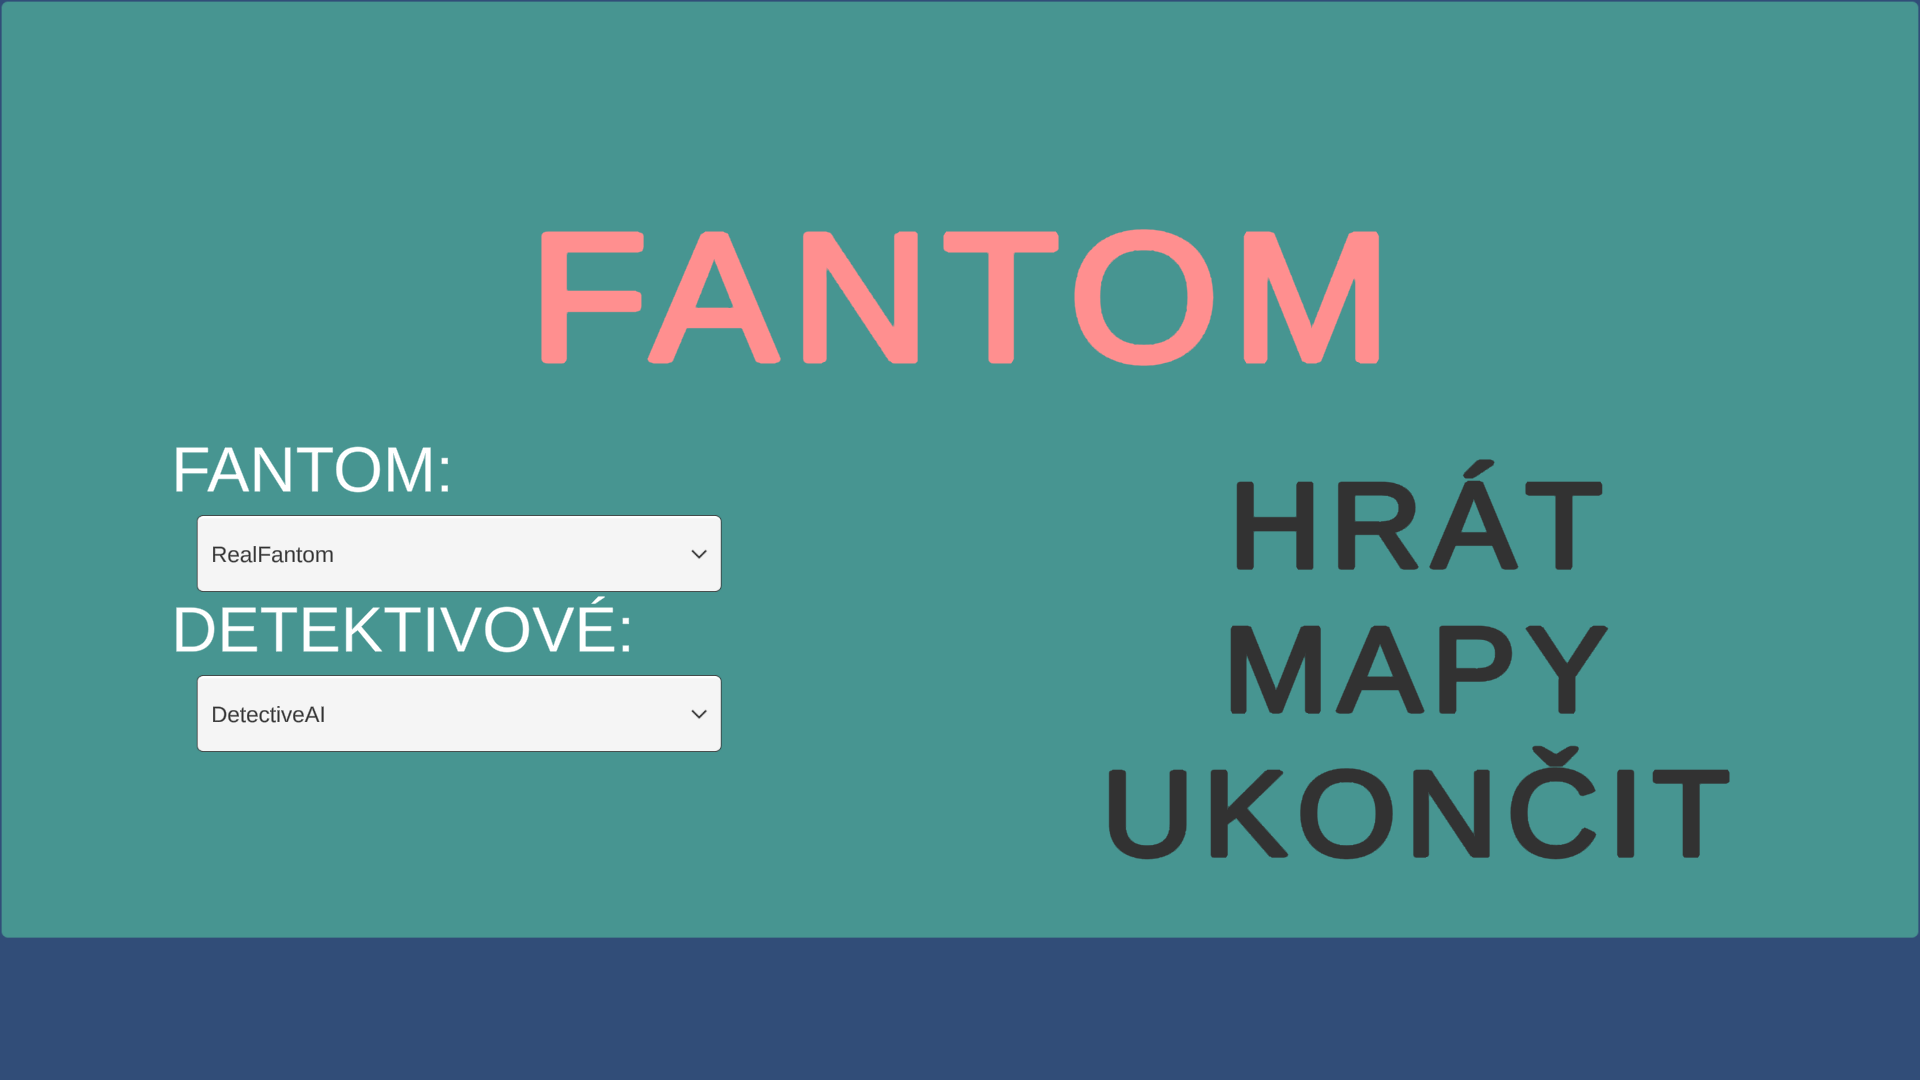
\includegraphics[width=1\textwidth]{main_menu.png}
  \caption{Hlavní menu}
  \label{fig:main_menu}
\end{figure}

\begin{figure}[h]
  \centering
  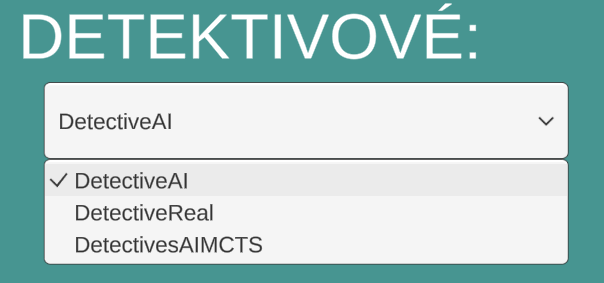
\includegraphics[width=1\textwidth]{player_selector.png}
  \caption{Výběr hráče}
  \label{fig:player_selector}
\end{figure}
\clearpage
\subsubsection{Herní obrazovka}

Při hře vidí hráč mapu hry a důležité informace o hře viz Obrázek~ \ref{fig:ingame_view}. Vlevo nahoře se nachází aktuální kolo, kdo je na tahu (Fantom či detektiv) a tlačítko "Schovat Fantoma", které pouze zneviditelní či naopak ukáže Fantoma, je určeno pro hraní dvou lidí proti sobě, pro hraní s umělou inteligencí se nedoporučuje využívat. Vlevo dole jsou dvě tlačítka, "Všechny žetony", které zobrazí tabulku s počtem aktuálních žetonů dopravních prostředků pro každého hráče, a "Fantom tahy" zobrazující historii Fantomových tahů, která se objeví vpravo, aktuálně je zobrazená. Vpravo dole jsou tři tlačítka pro dopravní prostředky, pomocí kterých se hráč, zvolil-li si ovládání Fantoma či detektivů a je právě na tahu, vybírá dopravní prostředek na cestování. Po zvolení dopravního prostředku se zvýrazní možné tahy žlutým kruhem (ukázka po zvolení Tramvaje na Obrázku~\ref{fig:ingame_view})

\begin{figure}[h]
  \centering
  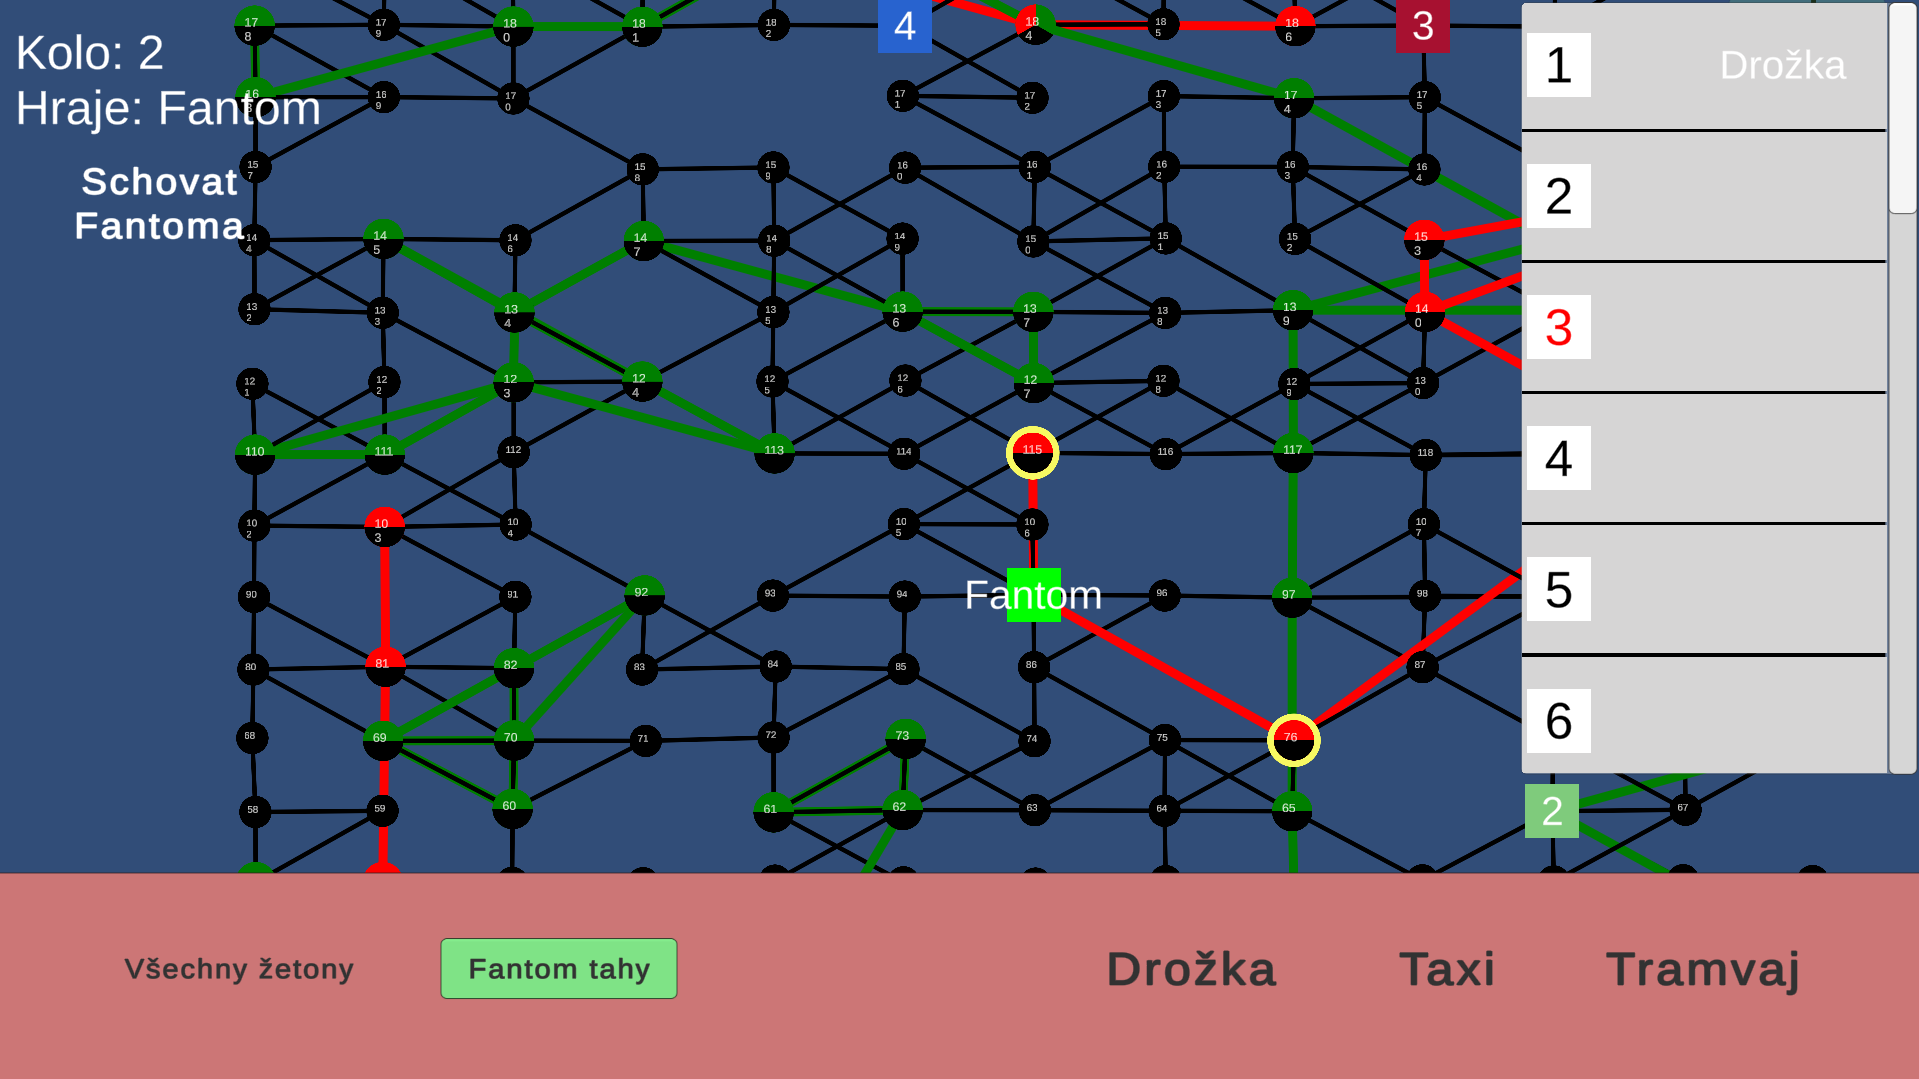
\includegraphics[width=1\textwidth]{ingame_view.png}
  \caption{Pohled při hře, vpravo historie tahů Fantoma}
  \label{fig:ingame_view}
\end{figure}
\clearpage
\subsubsection{Konec hry}

Po dohrání hry se objeví menu nabízející ukončení hry pomocí "UKONČIT", hrát znovu pomocí "HRÁT ZNOVU" a uložení mapy do správného JSON formátu mezi soubory hry pomocí "ULOŽIT MAPU" (Obrázek~\ref{fig:end_menu}).

\begin{figure}[h]
  \centering
  
\includegraphics[width=0.8\textwidth]{end_menu.png}
  \caption{Menu po dohrání hry}
  \label{fig:end_menu}
\end{figure}

\section{Instalace hry}

Vše potřebné zajistí k práci přiložený FantomInstaller.exe. Vytvoří novou složku s hrou ve stejné složce, ve které se nachází. Hra je spustitelná pomocí souboru ``Fantom.exe''.

\chapter{Experimenty}

\section{Druhy experimentů}

Experimenty začnu porovnáním náhodného hráče proti hráči využívajícím heuristiku pro rozhodování, dle \cref{sub:fantomai} a \cref{sub:detectivesai}. Lepší z těchto dvou hráčů, tj. ten který vyhraje více her, postoupí a odehraje další hry proti hráči, který využívá ISMCTS, dle mé implementace ze \cref{sec:impl}. Úvodní zápasy budou hrány v obou možnostech, tj. Fantom náhodný hráč proti detektivům s heuristikou a Fantom s heuristikou proti náhodným detektivům. Celý turnaj bude proveden na třech různých mapách.

Parametry hry jsou předem stanovené. Délka hry je 24 kol. Kola, kdy se Fantom musí ukázat jsou následující: 3., 8., 13., 18. a 21. Úvodní žetony každého detektiva jsou: drožka 10krát, taxi 9krát a tramvaj 5krát, úvodní žetony Fantoma jsou: drožka 
4krát, taxi 3krát a tramvaj 3krát. Všechny souboje provedu 50krát. V každém tahu má hráč s Monte Carlo technikami pro nalezení akce nastavenou délku simulování na 2,5 sekundy. Vyšší čas nabízí větší množství simulací, čímž by mohl být odhad nejlepší akce vylepšen. 

\section{Použité mapy}

Zvolené mapy, Obrázky \ref{fig:map1}, \ref{fig:map2} a \ref{fig:map3}, jsou náhodně vygenerované z implementace hry. Kvůli náhodnému generování mohou často vznikat mapy výhodné pro jednu stranu. Výběr map nedoprovázelo testování férovosti, experimenty popisují funkčnost v prostředí hry. 

\begin{figure}[h]
  \centering
  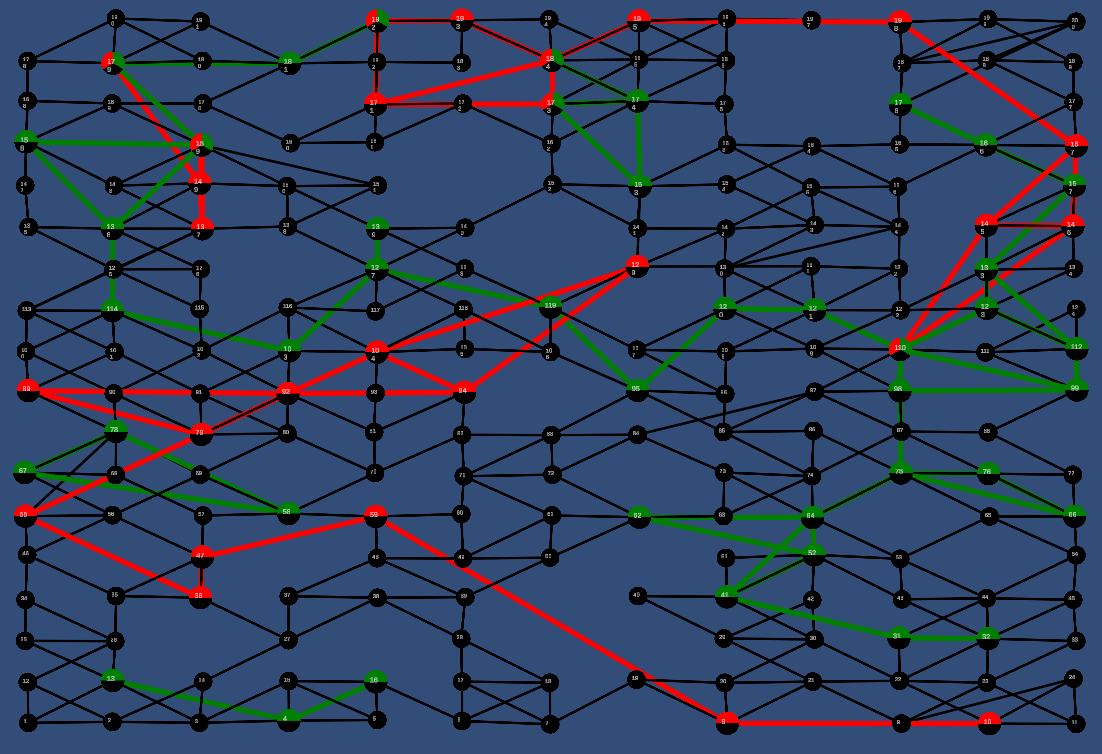
\includegraphics[width=1\textwidth]{mapa1.png}
  \caption{Mapa 1}
  \label{fig:map1}
\end{figure}

\begin{figure}[h]
  \centering
  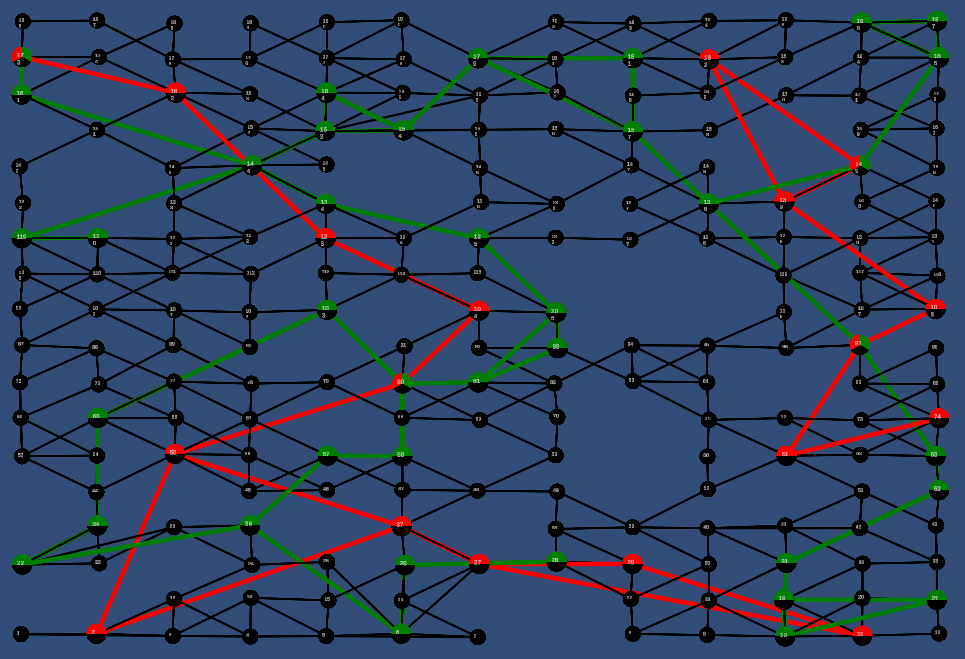
\includegraphics[width=1\textwidth]{mapa2.png}
  \caption{Mapa 2}
  \label{fig:map2}
\end{figure}

\begin{figure}[h]
  \centering
  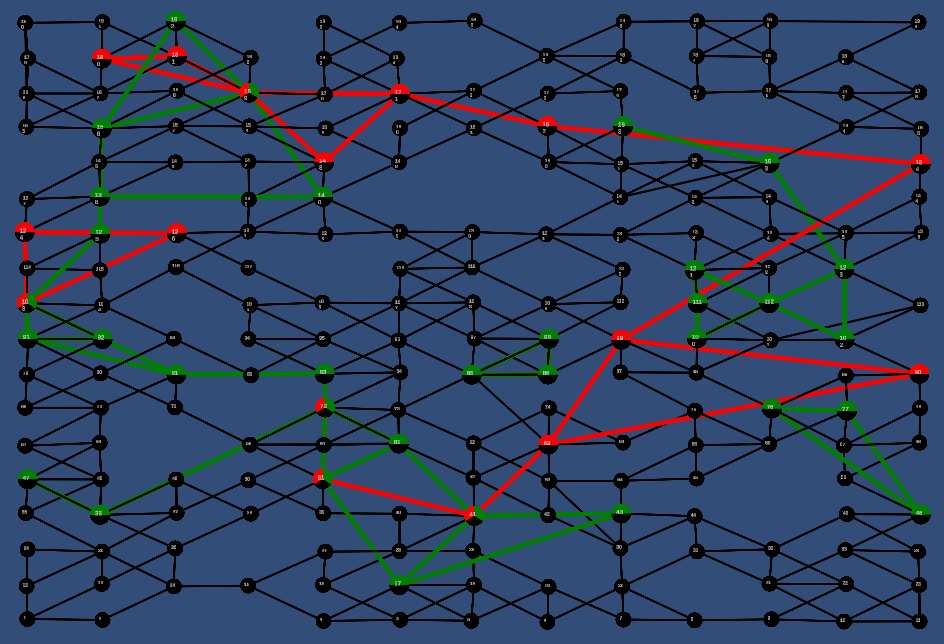
\includegraphics[width=1\textwidth]{mapa3.png}
  \caption{Mapa 3}
  \label{fig:map3}
\end{figure}
\clearpage

\section{Náhodný proti heuristice}
Nejdříve se proti sobě utkají náhodný hráč s hráčem využívající heuristiky dle \cref{sub:fantomai} a \cref{sub:detectivesai}. Náhodný hráč samozřejmě nijak nevyužívá znalosti a vlastnosti hry. Naopak hráč využívající heuristiku se snaží použít nejlepší možný tah s aktuálními znalostmi.

Z výsledků v tabulkách \ref{tab:heur-rand} a \ref{tab:rand-heur} je očividné, že se vyplatí využívat známé informace místo náhodného chození po mapě. Přesto se detektivům, kteří využívají heuristiku, daří proti náhodnému hráči více než Fantomovi. Detektivové s heuristikou neprohráli ani jednu hru. Důvodem nejspíše bude, že Fantom chce pro výhru využívat neznalosti detektivů, také náhodnými pohyby nijak netrestá vlastnosti heuristiky detektivů - směřují pouze k poslednímu známému místu Fantoma, jelikož se může zdržovat dlouze v blízkém okolí.

Na histogramech \ref{fig:hist-heur-rand} a \ref{fig:hist-rand-heur} je zobrazená četnost výherních kol z pohledů detektivů přes všechny tři testované mapy. 

Detektivové hrající náhodně proti chytřejšímu hráči využívající heuristiky, Obrázek \ref{fig:hist-heur-rand}, vyhrávali většinou díky náhodnosti prvního kola Fantoma - první tah volí čistě náhodně. V pozdějších kolech se díky heuristice Fantom mohl detektivům vyhýbat. Oproti tomu detektivové hrající dle heuristiky, Obrázek \ref{fig:hist-rand-heur}, nejčastěji vyhráli v prvních 12ti kolech. Heuristika je proti náhodnému hráči dostatečně silná, že náhodný Fantom skoro nikdy nevyhraje.

\begin{table}[htbp]
    \centering
    \caption{Počet výher detektivů (náhodný) a Fantoma (heuristika)}
    \label{tab:heur-rand}
    \begin{tabular}{@{}lcc@{}}
        \toprule
        \textbf{Mapa} & \textbf{Detektivové} & \textbf{Fantom} \\
        \midrule
        Mapa 1 & 9 & 41 \\
        Mapa 2 & 5 & 45 \\
        Mapa 3 & 4 & 46 \\
        \bottomrule
    \end{tabular}
\end{table}

\begin{table}[htbp]
    \centering
    \caption{Počet výher detektivů (heuristika) a Fantoma (náhodný)}
    \label{tab:rand-heur}
    \begin{tabular}{@{}lcc@{}}
        \toprule
        \textbf{Mapa} & \textbf{Detektivové} & \textbf{Fantom} \\
        \midrule
        Mapa 1 & 50 & 0 \\
        Mapa 2 & 50 & 0 \\
        Mapa 3 & 50 & 0 \\
        \bottomrule
    \end{tabular}
\end{table}

\begin{figure}[h]
  \centering
  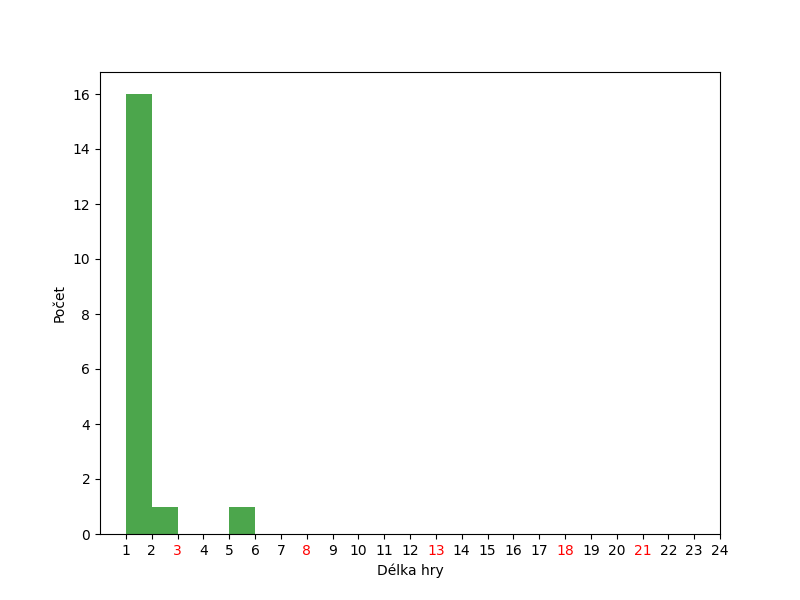
\includegraphics[width=0.85\textwidth]{heur-rand-histogram.png}
  \caption{Histogram délky her, kdy vyhráli detektivové. Fantom (heuristika) vs. detektivové (náhodný).}
  \label{fig:hist-heur-rand}
\end{figure}

\begin{figure}[h]
  \centering
  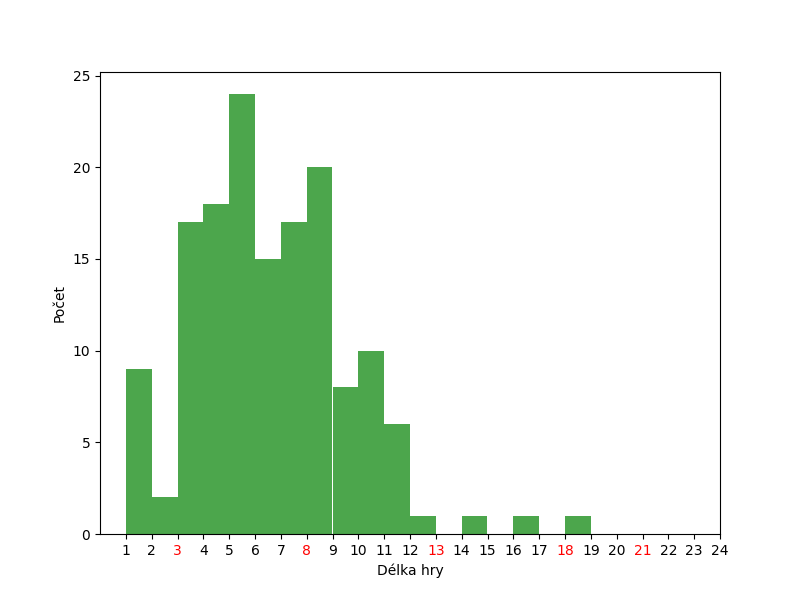
\includegraphics[width=0.85\textwidth]{rand-heur-histogram.png}
  \caption{Histogram délky her, kdy vyhráli detektivové. Fantom (náhodný) vs. detektivové (heuristika).}
  \label{fig:hist-rand-heur}
\end{figure}

\clearpage


\section{Heuristika proti ISMCTS}
Proti hráči využívající ISMCTS se utká hráč využívající heuristiku - výherce předešlého kola. Hráč se pomocí ISMCTS snaží simulovat průběhy her a ze simulací odvodit nejlepší tah.   

Na histogramech \ref{fig:hist-mcts-heur} a \ref{fig:hist-heur-mcts} je zobrazená četnost výherních kol z pohledů detektivů přes všechny tři testované mapy. 

Ve hrách, kdy Fantom využívá ISMCTS proti detektivům s heuristikou, Obrázek \ref{fig:hist-mcts-heur}, vychází, že detektivové nejčastěji vyhrají kolem poloviny délky hry - mezi 7. a 18. kolem. Oproti náhodnému Fantomovi trvá detektivům déle, než se jim podaří Fantoma dopadnout. Pokud se hra dostane do posledních kol, je možné, že detektivům také dochází žetony a přichází o možnosti dopadení Fantoma. Oproti tomu detektivové využívající ISMCTS proti Fantomovi s heuristikou hrají hůře, Obrázek \ref{fig:hist-heur-mcts}. Nejčastěji vyhrají díky náhodnému prvnímu kolu heuristiky, jinak v průběhu hry vyhrávají spíše ve druhé polovině.

\begin{table}[htbp]
    \centering
    \caption{Počet výher detektivů (heuristika) a Fantoma (ISMCTS)}
    \label{tab:mcts-heur}
    \begin{tabular}{@{}lcc@{}}
        \toprule
        \textbf{Mapa} & \textbf{Detektivové} & \textbf{Fantom} \\
        \midrule
        Mapa 1 & 17 & 33 \\
        Mapa 2 & 20 & 30 \\
        Mapa 3 & 19 & 31 \\
        \bottomrule
    \end{tabular}
\end{table}

\begin{table}[htbp]
    \centering
    \caption{Počet výher detektivů (ISMCTS) a Fantoma (heuristika)}
    \label{tab:heur-mcts}
    \begin{tabular}{@{}lcc@{}}
        \toprule
        \textbf{Mapa} & \textbf{Detektivové} & \textbf{Fantom} \\
        \midrule
        Mapa 1 & 4 & 46 \\
        Mapa 2 & 9 & 41 \\
        Mapa 3 & 2 & 48 \\
        \bottomrule
    \end{tabular}
\end{table}


\begin{figure}[h]
  \centering
  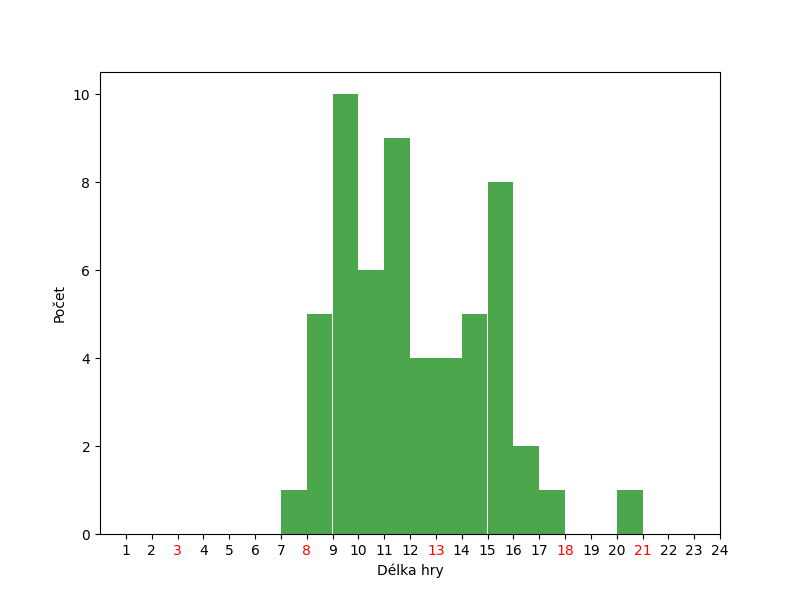
\includegraphics[width=0.85\textwidth]{mcts-heur-histogram.png}
  \caption{Histogram délky her, kdy vyhráli detektivové. Fantom (ISMCTS) vs. detektivové (heuristika).}
  \label{fig:hist-mcts-heur}
\end{figure}

\begin{figure}[h]
  \centering
  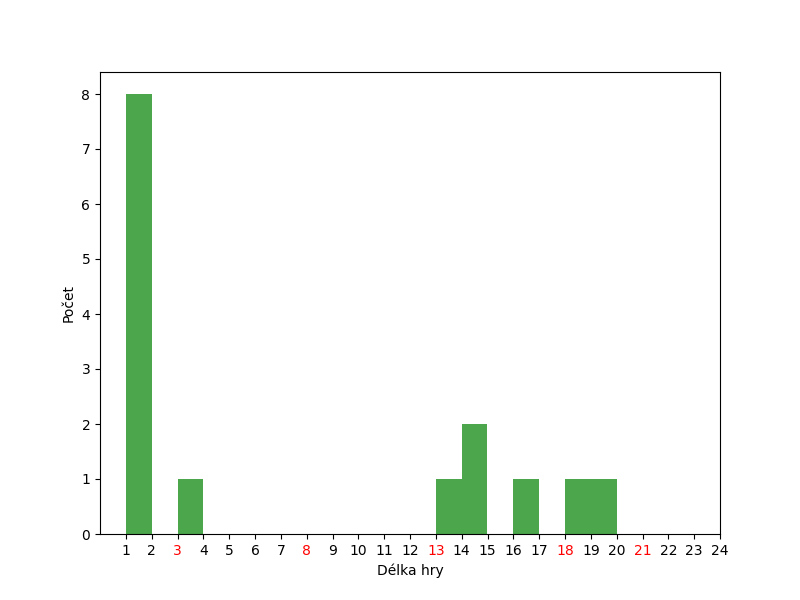
\includegraphics[width=0.85\textwidth]{heur-mcts-histogram.png}
  \caption{Histogram délky her, kdy vyhráli detektivové. Fantom (heuristika) vs. detektivové (ISMCTS).}
  \label{fig:hist-heur-mcts}
\end{figure}

Z výsledků v tabulkách \ref{tab:mcts-heur} a \ref{tab:heur-mcts} vyplývá, že Fantom využívající ISMCTS je lepší než hráč s heuristikou. Proti tomu, detektivové využívající ISMCTS dosahují velmi nízké úspěšnosti. Proti Fantomovi s heuristikou vyhrají méně než 10 \% her. 

Důvodů může být několik. Jedním z možných problémů je již zmíněný {\it strategy fusion} \cite{Soete2013MonteCarloTS}, který popisuje situaci, kde se algoritmus pokusí najít nejlepší strategii pro každou determinizaci zvlášť, místo hledání nejlepší strategie pro všechny determinizace zároveň. Proti Fantomovi používají detektivové 5 figurek, mají tedy řádově více možných akcí.

\clearpage
\section{Možná vylepšení ISMCTS}

Zlepšení algoritmu může poskytnout kvalitnější strategie, například se toho dá dosáhnout zefektivněním implementace algoritmu. Jiným způsobem je využít znalost domény hry. Zabudovat znalosti lze několika způsoby. Například je možné determinizace vybírat nikoliv uniformě z informačního stavu, ale podle pravděpodobnostní distribuce určující pravděpodobnost každého stavu. Pravděpodobnější determinizace budou častěji zvoleny a budou mít možnost více ovlivnit získanou strategii. Při iteraci je možné zvolit chytřejší simulační (rollout) strategii, která reprezentuje chování chytřejšího hráče místo náhodného.  

\section{Možná vylepšení heuristiky}
Zlepšení výsledků je možné dosáhnout upravením heuristiky pro první kolo. Kdyby v prvním kole nebyl výběr náhodný, bude hráč silnější. Například Fantom využívající heuristiky velmi často prohrál v prvním kole proti detektivům s~ISMCTS, histogram \ref{fig:hist-mcts-heur}.

\section{Závěr experimentů}
Vidíme, že mapy a parametry hry jsou nastaveny tak, že detektivové i Fantom mají naději na výhru. Záleží na jejich strategii a strategii oponenta. Navržení umělí hráči, využívající heuristiky či ISMCTS, poskytují škálu různě silných soupeřů pro lidského hráče.  


\chapwithtoc{Závěr}
V rámci práce jsem implementoval hru na motivy Fantom staré Prahy a dva druhy umělých agentů a popsal základy teorie her a některé jejich aplikace. Popis dvou souvisejících bakalářských prací a velmi aktuálního článku mi poskytl zajímavé poznatky a vhled do řešení daného problému.

Implementoval jsem hru v herním engine Unity. Součástí práce je i hra samotná a její popis. Pro vývoj hry bylo potřebné získat znalosti o herním engine Unity a aplikovat je. 

Hlavním cílem této práce bylo implementovat algoritmus umělé inteligence do hry. V rámci práce jsem implementoval dva druhy umělých agentů. První využívá heuristiky vymyšlené na základě domény hry, druhý naopak využívá Monte Carlo techniky v algoritmu Information Set Monte Carlo Tree Search (ISMCTS), které přímo nevyužívají žádné znalosti domény. 

Pro otestování funkčnosti a úrovně umělých inteligencí jsem připravil menší turnaj. V prvním kole se utkala umělá inteligence využívající heuristiku proti náhodnému hráči. Heuristika vyhrála v obou případech, jak za Fantoma, tak za detektivy. Ve druhém kole se vítěz prvního kola utkal s~hráčem používajícím ISMCTS. Výsledky byly smíšené, za Fantoma vyhrál hráč s~ISMCTS, za detektivy naopak heuristika. Celý turnaj probíhal na třech různých mapách, v každém kole se provedlo 50 her pro obě možnosti umělých inteligencí.

Z výsledků experimentů vidíme, že umělí hráči hrají se snahou vyhrát. Díky výhrám na obou stranách můžeme usoudit, že zvolené mapy a parametry umožňují vyhrát jak Fantomovi, tak detektivům. Výherce je hráč s lepší strategií vůči jeho oponentovi. Algoritmus ISMCTS, který je nejen složitý, ale i aktuální, se prokázal být funkčním.

Implementace hry nabízí možnost za Fantoma i detektivy zvolit reálného i umělého hráče, umožňuje tedy hrát lidským hráčům proti sobě, ale i proti různě silným soupeřům umělé inteligence.
\include{bibliography}

\appendix
%\include{howto}
\chapter{Programátorská
dokumentace}\label{programuxe1torskuxe1-dokumentace}

\section{Graf}\label{graf}

Třída ``GameGraphScript'' je klíčovým prvkem herního prostředí,
zajišťujícím řízení interakcí mezi herním grafem a jeho uzly. Zodpovídá
za generování grafu na základě nových nebo existujících dat, přiřazování
identifikátorů uzlů, jejich vizuální reprezentaci a generování hran mezi
nimi. Umožňuje ukládání dat grafu a nabízí funkci hledání nejkratší
cesty mezi uzly (BFS).

\subsection{Vrchol}\label{vrchol}

Třída ``GameNodeScript'' je klíčovým prvkem herního prostředí,
zodpovědným za reprezentaci uzlů v herním grafu, jejich vizuální
zobrazení a interakci. Umožňuje nastavovat ID, pozici, spojené uzly a
transportní typy, a dále provádět ověřování spojení, manipulovat se
zvýrazňovačem a volat logiku na základě interakce. Struktura
``NodeData'' slouží k ukládání informací o uzlech.

\subsection{Hrana}\label{hrana}

Třída ``GameEdgeScript'' pouze drží texturu, kterou LineRenderer
vykreslí.

\section{Herní logika}\label{hernuxed-logika}

Třída ``GameLogicScript'' představuje jádro herní logiky a spravuje
průběh hry, interakce mezi hráči a grafem hry. Obsahuje odkazy na různé
herní komponenty, včetně grafu hry, správce historie Fantoma, ovladače
kamery, vykreslovače figurek, textu označujícího tah a panelu konce hry.
Třída řídí hráče a tahy, nastavuje viditelnost hráčů a tokenů,
implementuje vizuální efekty a animace tahu hráčů, spravuje informace o
poloze hráčů a tokeny, kontroluje podmínky ukončení hry a zajišťuje
hladký průběh herní smyčky. Kromě toho obsahuje metody pro správu konce
hry, zobrazuje konečný panel a ukládá statistiky. Třída také zahrnuje
utility pro správu cest k souborům.

\section{Config}\label{config}

Struktura ``Config'' zahrnuje několik vnořených struktur pro jednotlivé
konfigurační sekce. Každá konfigurační sekce obsahuje několik proměnných
s hodnotami nastavení. Metody BasicConfig, LoadConfig, LoadConfigOrBasic
a SeeStructure umožňují manipulaci s konfiguracemi.

\section{Logy}\label{logy}

Rozhraní ``IGameLogger'' definuje metody pro logování informací o
průběhu hry, chybách a dalších událostech.

Třída ``EmptyLogger'' implementuje rozhraní ``IGameLogger'' a všechny
logy zahazuje, tj. neprovádí žádnou skutečnou operaci.

Třída ``FileLogger'' také implementuje rozhraní ``IGameLogger'' a slouží
k logování informací do souboru. Konstruktor třídy ``FileLogger''
inicializuje logovací mechanismus a vytváří soubor, pokud neexistuje.
Metody LogTurn, LogError a LogInfo slouží k zaznamenávání různých typů
zpráv do souboru. Metody WriteLine a Write slouží k zápisu zpráv do
souboru, s ohledem na vláknovou bezpečnost pomocí uzamčení (lock).

\section{Ukládání map}\label{ukluxe1duxe1nuxed-map}

Třída ``MapData'' je odvozena od třídy ScriptableObject a slouží k
uchování dat mapy. Obsahuje informace o JSON datovém řetězci a zda je
mapa vybrána.

Struktura ``NodeDataHolder'' obsahuje informace o uzlech na mapě, včetně
jejich dopravních spojení a pozic.

Struktura ``StringPosition'' slouží k uchování pozice jako řetězce pro
JSON serializaci.

Struktura ``EnumIntPair'' uchovává páry klíč-hodnota, kde klíč je
celočíselný identifikátor a hodnota je seznam celočíselných hodnot.

Struktura ``EnumDictionary'' uchovává slovník, který mapuje klíče na
seznam hodnot.

Třída ``NodeConverter'' obsahuje metody pro konverzi instancí třídy
GameNodeScript na JSON. Tato třída umožňuje převést uzly mapy a seznam
uzlů na JSON formát.

\section{Generování map}\label{generovuxe1nuxed-map}

Rozhraní IGraphGenerator definuje metody pro generování uzlů a načítání
konfigurace.

Třída SimpleGraphGenerator implementuje rozhraní IGraphGenerator a
provádí generování uzlů a hran v grafu na základě zadané konfigurace.
Tato třída obsahuje metody pro generování uzlů, včetně zpracování
existujících uzlů a vytváření hran mezi nimi. Taktéž zde jsou
implementovány metody pro zpracování konfigurace a vytváření spojení
mezi uzly.

\section{Hráč}\label{hruxe1ux10d}

\subsection{AI}\label{ai}

Rozhraní ``IFantom'' a ``IDetectives'' slouží jako kontrakty pro hráče
Fantoma a detektivů. Obě tato rozhraní dědí od základního rozhraní
``IPlayerBase'', které obsahuje metody pro správu tahů, nastavení
dostupných transportních tokenů a reakci na tahy protivníka.

\subsection{Reálný hráč}\label{reuxe1lnuxfd-hruxe1ux10d}

Třída ``RealBase'' je abstraktní třídou pro reálné hráče a obsahuje
logiku pro reakci na kliknutí na herní uzel.

\subsection{Struktura Move}\label{struktura-move}

Struktura ``Move'' reprezentuje tah hráče a obsahuje informace o pozici
a druhu dopravního prostředku.

\subsection{Hledání hráčů}\label{hleduxe1nuxed-hruxe1ux10dux16f}

Třída ``PlayerFinder'' je utilitní třídou, která umožňuje nalézt typy
implementující dané rozhraní v určitém assembly. Obsahuje metodu
``GetTypesWithInterface'', která vrací seznam typů, které implementují
specifikované rozhraní ``T''. Dále obsahuje metodu
``GetClassNamesFromTypes'', která z kolekce typů získá seznam názvů
těchto typů.

Třída ``TypeLoaderExtensions'' obsahuje rozšíření pro načítání typů z
assembly. Metoda ``GetLoadableTypes'' umožňuje získat načitatelné typy z
dané assembly a zároveň zachytává výjimky, které mohou nastat během
načítání typů.

\section{Vykreslování postav}\label{vykreslovuxe1nuxed-postav}

Třída ``FigureRendererScript'' se stará o vykreslování a pohyb herních
figurek (detektivů a Fantoma). Figurky jsou reprezentovány pomocí
sprite a barev. Třída obsahuje metody pro inicializaci a přípravu
figurek, a také pro animovaný pohyb figurek na cílovou pozici.

Dále třída ``ColorUtility'' slouží pro operace spojené s barvami,
například pro výpočet podobnosti barev a zjišťování, zda je barva příliš
světlá pro bílý text.


\chapter{Uživatelská dokumentace}\label{uux17eivatelskuxe1-dokumentace}






% if your attachments are complicated, describe them in a separate appendix
%\include{attachments}

\openright
\end{document}
